%%%%%%%%%%%%%%%%%%%%%%%%%%% asme2ej.tex %%%%%%%%%%%%%%%%%%%%%%%%%%%%%%%
% Template for producing ASME-format journal articles using LaTeX    %
% Written by   Harry H. Cheng, Professor and Director                %
%              Integration Engineering Laboratory                    %
%              Department of Mechanical and Aeronautical Engineering %
%              University of California                              %
%              Davis, CA 95616                                       %
%              Tel: (530) 752-5020 (office)                          %
%                   (530) 752-1028 (lab)                             %
%              Fax: (530) 752-4158                                   %
%              Email: hhcheng@ucdavis.edu                            %
%              WWW:   http://iel.ucdavis.edu/people/cheng.html       %
%              May 7, 1994                                           %
% Modified: February 16, 2001 by Harry H. Cheng                      %
% Modified: January  01, 2003 by Geoffrey R. Shiflett                %
% Use at your own risk, send complaints to /dev/null                 %
%%%%%%%%%%%%%%%%%%%%%%%%%%%%%%%%%%%%%%%%%%%%%%%%%%%%%%%%%%%%%%%%%%%%%%

%%% use twocolumn and 10pt options with the asme2ej format

\documentclass[twocolumn,10pt]{asme2ej}

\usepackage[none]{hyphenat}
\usepackage{epsfig} %% for loading postscript figures
\usepackage{amsmath}
\usepackage{amssymb}
\usepackage{breqn}

% color code for matlab (thanks to SOUAD !)
\usepackage{listings} 
\lstset{language=Matlab}
\usepackage{color} %red, green, blue, yellow, cyan, magenta, black, white
\definecolor{mygreen}{RGB}{28,172,0} % color values Red, Green, Blue
\definecolor{mylilas}{RGB}{170,55,241}


\lstset{language=Matlab,%
   %basicstyle=\color{red},
   breaklines=true,%
   morekeywords={matlab2tikz},
   keywordstyle=\color{blue},%
   morekeywords=[2]{1}, keywordstyle=[2]{\color{black}},
   identifierstyle=\color{black},%
   stringstyle=\color{mylilas},
   commentstyle=\color{mygreen},%
   showstringspaces=false,%without this there will be a symbol in the places where there is a space
   numbers=left,%
   frame=trBL,
   numberstyle={\tiny \color{black}},% size of the numbers
   numbersep=9pt, % this defines how far the numbers are from the text
   emph=[1]{for,end,break},emphstyle=[1]\color{red}, %some words to emphasise
   %emph=[2]{word1,word2}, emphstyle=[2]{style},   
   }




\graphicspath{{./}{../CYLINDER/FIGURES/}}

% previous way
%\usepackage{listings}
\usepackage[colorlinks, linkcolor=blue, citecolor=blue,filecolor=black,urlcolor=blue]{hyperref}



\newcommand{\be}[1]{ \begin{equation} \label{#1}}
\newcommand{\ee}{\end{equation}}


\newcommand{\bes}[1]{ \begin{equation} \label{#1}\begin{array}{rl}}
\newcommand{\ees}{\end{array}\end{equation}}



%% The class has several options
%  onecolumn/twocolumn - format for one or two columns per page
%  10pt/11pt/12pt - use 10, 11, or 12 point font
%  oneside/twoside - format for oneside/twosided printing
%  final/draft - format for final/draft copy
%  cleanfoot - take out copyright info in footer leave page number
%  cleanhead - take out the conference banner on the title page
%  titlepage/notitlepage - put in titlepage or leave out titlepage
%  
%% The default is oneside, onecolumn, 10pt, final


%\title{Popularizing linear and nonlinear global approaches to hydrodynamic instabilities : 
%A review and a simple implementation for the wake of a cylinder}

\title{A practical review on linear and nonlinear global approaches to flow instabilities}

%%% first author
\author{D. Fabre$^{(a)}$,  V. Citro$^{(b)}$,  D. Ferreira Sabino$^{(a)}$, P. Bonnefis$^{(a)}$,  \& F. Giannetti$^{(b)}$
    \affiliation{
	$^{(a)}$ Institut de Mécanique des fluides de Toulouse (IMFT), University of Toulouse \\
	$^{(b)}$ Dipartimento do Ingegneria (DIIN), Universit\`a} di Salerno. 
}

%%% second author
%%% remove the following entry for single author papers
%%% add more entries for additional authors
%\author{V. Citro$^{(b)}$ \& F. Giannetti$^{(b)}$ \\
 %   \affiliation{ University of Salerno
  %  }
%}

\usepackage{cprotect}

\begin{document}
\lstset{numbers=left, numberstyle=\small, numbersep=8pt, frame = single, language=Matlab, framexleftmargin=15pt}

\maketitle    

%%%%%%%%%%%%%%%%%%%%%%%%%%%%%%%%%%%%%%%%%%%%%%%%%%%%%%%%%%%%%%%%%%%%%%
\begin{abstract}
{\it 
This paper aims at reviewing the linear and nonlinear approaches to study the stability of fluid flows. 
We provide a concise but self-contained exposition of the main concepts and specific numerical methods 
designed for global stability studies, including the classical linear stability analysis, the adjoint-based sensitivity and  
the most recent nonlinear developments. 
Regarding numerical implementation, a number of ideas making resolution particularly efficient are discussed, 
including mesh adaptation, simple shift-invert strategy instead of the classical Arnoldi algorithm, 
and a simplification of the recent nonlinear self-consistent approach proposed by Manti\v{c}-Lugo et al (2014). 
An open-source software implementing all the concepts discussed in the present paper is provided. 
The software is demonstrated for the reference case of the incompressible, two-dimensional flow around a circular cylinder, but is easily customisable to a variety of other flow configurations or flow equations.
%An abstract for an ASME paper should be less than 150 words and is normally in italics.
}
\end{abstract}

%%%%%%%%%%%%%%%%%%%%%%%%%%%%%%%%%%%%%%%%%%%%%%%%%%%%%%%%%%%%%%%%%%%%%%


\section{Introduction}

The concept of stability bears on the reaction of a system to a small perturbation of its state. If the generic disturbance grows in time, the system is unstable. The concept of stability can be simply formulated for a system of Ordinary Differential Equations (ODE). 
Such systems can be at equilibrium, where the state does not depend on time, or can present a periodic state, with all components returning to the same values, after every period. 

The stability of fluid flows usually depends on the value of a given parameter. A bifurcation occurs when a critical value is reached and the original solution becomes linearly unstable, with the system tending towards a new steady or unsteady state. 
In the second part of the 19th century, specific analytical and numerical methods able to study these bifurcations have emerged and are continuously evolving up to the present days. 
A crucial point, that drove the development in this field, is the availability of larger and larger computing resources. 
Initially, the linear stability theory focused on fluid flows that are homogeneous in two spatial directions, e.g. plane Poiseuille flow \cite{Dreid2004}. This implies that the streamwise and the spanwise base-flow gradients vanish and, as a consequence, it is possible to consider only one (streamwise) velocity component. Thus, the stability problem requires a \textit{local} numerical resolution, i.e. a one-dimensional problem.
On the other hand,  when there are at least two spatial variables, the class of methods suited to solve such problems are generally called {\em global stability approaches}.
A classical example of such behavior in fluid dynamics is the instability occurring in the wake of a circular cylinder. At low Reynolds number (precisely for $Re < 46.7$) the flow is steady and symmetric, but for larger values of Re a global instability arises in the flow field leading to the well-known von K\'arm\'an vortex alley. 
This flow configuration has served as a benchmark in the development of this class of methods.  
If one is only interested in predicting the stability or instability of a flow, it is enough to conduct a {\em linear stability analysis} which is the fundamental brick of global stability approaches. 
Beyond this simple question, in the past two decades, a number of extensions have been developed and popularized.  {\em Adjoint methods} are an important extension \cite{GiannettiLuchini},\cite{Marquet}; they can give insight into the sensitivity of the flow to intrinsic or extrinsic contributions. 
{\em Nonlinear stability approaches} \cite{MLugo2014}, \cite{SippLebedev} have also been developed in order to extend the range of applicability of the approach towards large amplitude perturbations.




The objective of the present work is to contribute to the popularization of such methods 
in two ways:
\begin{itemize}
\item
First, we give a concise but self-contained exposition of the main concepts and 
specific numerical methods pertaining to global stability, including basic linear stability, adjoint-based sensitivity, as well as the most recent nonlinear developments.
\item
Secondly we offer an open-source and user-friendly software called  {\em StabFem} %\cprotect 
\footnote{The StabFem software may be obtained at the following url : \\
\url{https://github.com/erbafdavid/StabFem}
%{\sf \color{blue} https://github.com/erbafdavid/StabFem}
} 
to perform such calculations. The software combines program written in both FreeFem++ and Matlab languages. 
FreeFem++ is used to generate and adapt the meshes and to solve the various linear problems arising in the analysis. Matlab is used as a driver to monitor the computations, perform the required loops over parameters, and plot the results.
\end{itemize}

In the present paper the concepts are introduced and the software is demonstrated for the reference case of the incompressible, two-dimensional flow around a cylinder, but the software is easily customizable to a variety of other situations (compressible, three-dimensional, etc..).

Although we don't claim to invent any radically new method, our exposition and implementation contains a number of originalities making the computation particularly efficient in terms of computational time and memory\footnote{All the figures contained in the present paper can be processed by launching a single Matlab script {\sf SCRIPT\_CYLINDER\_ALLFIGURES.m} . On a MacbookPro (2018,  2.5Ghz, 16Go Ram) in single-core sequential execution,  and using mesh ${\mathbf M}_2$ as described in appendix B, the execution time is 203 seconds for the linear analysis (section 3), and 413 seconds for the nonlinear analysis.}.
% 1868 seconds using mesh M4
The most notable originalities are the systematic use of mesh adaptation (\S 2 and 3), the use of simple shift-invert instead of Arnoldi (\S 3), and a reformulation and simplification of the nonlinear self-consistent approach of Mantic-Lugo et al  (\S 4).
 

%which is based on both FreeFem++ and Matlab.
%The fundamental case of a cylinder is used as a guideline to present the method, but the 
%provide a simple and all-in-one implementation of 

\section{Linear stability analysis : equations and methods}
\vspace{.2cm}

\subsection{Computing a base-flow with Newton iteration}
\vspace{.2cm}

\paragraph{Navier-Stokes equations and weak form}

We start from the general problem of a flow field $[{\bf u},p]$ satisfying the incompressible Navier-Stokes equations on a domain $\Omega$,
\begin{eqnarray} \label{NSprimitive}
\partial_t {\bf u} = {\cal NS} ({\bf u},p)
\equiv - {\bf u} \cdot \nabla {\bf u} - \nabla p + \frac{2}{Re}  \nabla \cdot {\mathsf{D}}({\bf u}),  \\
\nabla \cdot {\bf u} = 0,
\end{eqnarray}
with suitable boundary conditions on the frontier $\partial \Omega$ of the domain.
Here $ {\mathsf{D}}({\bf u}) $ is the rate-of-strain tensor defined as
$$
 {\mathsf{D}}({\bf u}) = 1/2
\left( \nabla {\bf u} +  \nabla^T  {\bf u}\right),
$$ 
In the framework of finite element methods, we need to write the equation in weak form.
Prior to this we define a scalar product as follows, for either scalar or vectorial quantities 
$\left< \phi_1, \phi_2 \right> $:
$$
\left< \phi_1, \phi_2 \right> = \int_\Omega \overline{\phi}_1 \cdot \phi_2   \mbox{ d} \Omega,
$$
The weak form of the Navier-Stokes equations is readily defined by introducing test functions 
$[{\bf v},q]$ associated with the momentum and continuity equations, and integrating over the domain\footnote{In the simple presentation given here we have omitted the issue of boundary conditions. Details on way boundary conditions can be incorporated in the weak formulation through integration by parts can be found in appendix D.}
\be{NSweak}
\forall [{\bf v},q], \quad \partial_t \left< {\bf v}, {\bf u}\right> = \left< {\bf v} , {\cal NS} ({\bf u},p) \right> + \left< q, \nabla \cdot {\bf u}\right>.
\ee





\paragraph{Newton iteration}


We look for a steady base-flow $[{\bf u}_b,p_b]$ satisfying the steady Navier-Stokes equations, i.e. 
%${\cal NS} ({\bf u}_b,p_b) = 0$.
${\cal NS} ({\bf u}_b,p_b) = 0$.
Suppose that we have a {\em guess}  for the base flow $[{\bf u}_b^g,p_b^g]$  which almost satisfies the equations.  We look for a better approximation under the form
\be{Newton1}
[{\bf u}_b,p_b]  = [{\bf u}_b^g,p_b^g] + [\delta {\bf u}_b, \delta p_b].
\ee
Injecting (\ref{Newton1}) into the weak form (\ref{NSweak}) of the Navier-Stokes equations and linearizing leads to  
${\cal NS}  ({\bf u}_b^g,p_b^g) +  {\cal LNS} _{{\bf u}_b^g}(\delta {\bf u}_b,\delta p_b)$, which can also be written in weak form as :
\bes{Newton2}
&\left< {\bf v}, {\cal NS} ({\bf u}_b^g,p_b^g)\right> + \left<q, \nabla \cdot {\bf u}_b^g\right>  
\\
+ &\left< { \bf v}, {\cal LNS} _{{\bf u}_b^g}( \delta {\bf u}_b,\delta p_b) \right> + \left<q, \nabla \cdot \delta{\bf u}_b\right> = 0,
\ees
where ${\cal LNS}$ is the linearised Navier-Stokes operator, defined by its action on a flow field $[{\bf u} , p]$ as follows 
\be{defNSL}
 {\cal LNS}_{{\bf U}}( {\bf u}, p) = - {\cal C}( {\bf U} , {\bf u}) -\nabla p
+\frac{2}{Re} \nabla  \cdot {\mathsf{D}}({\bf u}), %\quad ( \mbox{ with } \nabla \cdot {\bf u } = 0 \, ).
 \ee
and ${\cal C}$ is the convection operator defined by 
\be{defC}
{\cal C}( {\bf U} , {\bf u}) = \left( {\bf U} \cdot \nabla \right) {\bf u} + \left( {\bf u} \cdot \nabla \right)  {\bf U}.
\ee
This problem can now be discretized by projecting upon a basis of Taylor-Hood $(u,v,p) \rightarrow (P2,P2,P1)$ finite elements. Noting $\delta X$ the discretization of $[\delta {\bf u}_b,\delta p_b]$ this eventually leads to a matricial problem of the form $A \cdot \delta X = Y$. The procedure of Newton iteration is to solve iteratively this set of equations up to convergence.
In our implementation, the algorithm is written in the Freefem++ solver {\em Newton\_2D.edp} 
which is wrapped by the Matlab driver {\sf SF\_BaseFlow.m}.

\subsection{Linear stability}
\vspace{.2cm}

\paragraph{Direct eigenvalue problem}
We study the onset of the instability within the linear theory by using a normal-mode analysis:
\be{startmodepropre}
{\bf u} ({\bf{x}},t) = {\bf u}_b({\bf{x}}) + \epsilon \hat{\bf u}({\bf{x}}) e^{\lambda t}, \,\,\,\, {p}({\bf{x}},t) = {p}_b({\bf{x}}) + \epsilon \hat{p}({\bf{x}}) e^{\lambda t},
\ee
where $\lambda = \sigma + i \omega$ is the eigenvalue, $\sigma$ the amplification rate,
$\omega$ the oscillation rate, $\hat{{\bf u}},\hat{p}$ the eigenmodes, and $\epsilon$ a small parameter.
The eigenmodes and the eigenvalues are the solution of the following eigenproblem:
 \be{LEP}
\lambda \hat{{\bf u}} = {\cal LNS}_{{\bf u}_b}( \hat{\bf u},\hat{p}),
\ee
or, in weak form : 
\be{eigenvalueproblem}
\lambda \left< {\bf v} , \hat{{\bf u}} \right> = \left< {\bf v}, {\cal LNS}_{{\bf u}_b} ( \hat{\bf u},\hat{p})\right> + \left< q, \nabla \cdot \hat{\bf u} \right>.
\ee
After discretization, we end up with an eigenvalue problem with the matricial form
\be{Eigen_matricial}
\lambda {\mathsf{B}} \hat{X} = {\mathsf{A}} \hat{X},
\ee
where ${\mathsf{A}}$ is the matrix resulting from the discretization of ${\cal LNS}_{{\bf u}_b}$, i.e. the same matrix  appearing in the Newton computation of the base flow, and  $B$ is a weight matrix associated to the scalar product $\left<v,u\right> = \int \overline{\bf v} \cdot {\bf u} \mbox{ d} \Omega$.

\paragraph{Adjoint eigenvalue problem and structural sensitivity}
Developed in the two past decades, the concept adjoint modes has now become an unavoidable complement to the linear global stability approach. We here give a short summary of the definition and usefulness of this concept, 
we refer to Luchini \& Bottaro\cite{LucBott2014} for further details.
First of all, the {\em adjoint linearised Navier-Stokes operator} ${\cal LNS}^\dag$ is defined thanks to the following 
property:
\bes{NSLAdj}
\forall ( {\bf u}, p ; {\bf v}, q), & \left< {\cal LNS}^\dag_{\bf U}( {\bf v},q) ,{\bf u}\right> + \left< \nabla \cdot {\bf v},p\right>  \\
=& \left< {\bf v}, {\cal LNS}_{\bf U} ({\bf u},p)\right> + \left< q, \nabla \cdot {\bf u}\right>.
\ees
We can then define the adjoint eigenvalues and eigenmodes as the solutions of the eigenvalue problem 
\be{EigenAdj} 
\forall ( {\bf u}, p), \quad  \lambda^\dag \left< \hat{\bf v}, {\bf u}\right> =
 \left< {\cal LNS}^\dag_{\bf U}( \hat{\bf v},\hat{q}) ,{\bf u}\right> + \left< \nabla \cdot \hat{\bf v},p\right> . 
\ee
It can be shown \cite{SchmidHenningson2001} that the adjoint eigenvalues $\lambda^\dag_k$ are the complex conjugates of the direct eigenvalues $\lambda_k$. 

Although the concept of adjoint operator may sound complicate, the resolution of the adjoint problem using finite elements methods is actually extremely easy. In effect, the scalar product used in the definition of the weak formulation and that appearing in the definition of adjoint being the same, the weak formulations of both problems are thus identical when exchanging the test functions and the unknown functions. Thus the matricial form of the discretized version of (\ref{EigenAdj}) is deduced from the one of the direct problem by a simple (Hermitian) transpose of the matrix :
\be{Eigen_Adj_matricial}
\overline{\lambda}^\dag B \hat{X}^\dag = A^T \hat{X}^\dag.
\ee
Adjoint eigenmodes are a powerful tool for investigating problems such as receptivity, transient growth, control and sensitivity (see the reviews of \cite{Jmc2005}, \cite{Ps2007}, \cite{LucBott2014}). The simplest physical interpretation of an adjoint eigenmode is as follows : it corresponds to the initial condition which has maximum projection along the direction of the corresponding eigenmode.
Thus, the adjoint of the most amplified mode corresponds to the optimal perturbation which will maximize the growth of energy in the limit of large time. In effect, one can prove that for $t \rightarrow \infty$  the asymptotic behaviour of a solution with initial condition ${\bf u}_i$  is given as :
$$
{\bf u}(t) \approx 
\frac{ \left< \hat{\bf u}^\dag, {\bf u}_i\right>}{\left<\hat{\bf u}^\dag, \hat{\bf u}\right>} 
e^{\lambda t} \hat{\bf u}.
$$
The choice ${\bf u}_i = \hat{\bf u}^\dag$ is the initial condition of norm unity which maximizes the first factor in this expression.

The adjoint eigenmode also allows us to introduce the so-called {\em structural sensitivity tensor } that is defined as 
\be{Structursens} 
{\bf{S}}({\bf{x}}) = \frac{|| \hat{\bf u}^\dag|| \,\, ||\hat{\bf u}|| }{{\left<\hat{\bf u}^\dag, \hat{\bf u}\right>}},
\ee 
which has became popular in the recent years.
%is called the structural sensitivity of the eigenmode. 
This quantity is a direct and practical measure of the effect of perturbations of the linear operator on the eigenvalue. The region of the flow where ${\bf{S}}({\bf{x}})$ reaches its maximum values is, thus, the region where the instability mechanism originates, and is often referred to as the {\em wavemaker region}.

%\end{itemize}

\paragraph{Iterative methods for eigenvalue computations}

The numerical resolution of generalized eigenvalue problems such as $A X = \lambda B X$ (or its adjoint version (\ref{Eigen_Adj_matricial}) ), 
can be performed using several methods. Direct methods to compute the whole spectrum are both costly prohibitive and useless. A popular alternative is the use of iterative methods to compute a limited set of eigenvalues located in the vicinity of a 
{\em shift} value $\lambda_{shift}$. The simplest version of this method is the simple shift-invert iteration, which consists of solving iteratively the system
$$
X^{n} =  (A- \lambda_{shift} B)^{-1} B X^{n-1}.
$$ 
It is easy to show that this iterative procedure quickly asymptotes to $X^{n+1} \approx ({\lambda^*}^{-1})^n \hat{X}$
where $\hat{X}$ is the eigenmode with largest ${\lambda^*}^{-1}$ (i.e. the one with eigenvalue $\lambda$ closest to the shift). 


When a good estimation of the eigenvalue is available, this method converges very rapidly and is very efficient, but it can only provide a single eigenvalue.
If we want to compute a larger number of eigenvalues, we can revert to a generalized version of iterative methods, called Arnoldi methods\cite{Arnoldi51}. The shift-invert version of the Arnoldi method is in fact the most commonly used method of the current time and is at the basis of both the popular matlab function {\tt{eigs}} and the eigenvalue solver of FreeFem (i.e. ARPACK++). Our implementation in StabFem allows to chose between single eigenvalue computation (power method) and multiple eigenvalue computation (Arnoldi). The selection is made according to the parameter \verb|nev|  (i.e. number of requested eigenvalues) transmitted to the driver.



\begin{figure*}[t]
\small
\lstinputlisting{Script_Cylinder_Part1.m}
 \normalsize
\caption{Illustration of the usage of the StabFem software to produce an adapted mesh and study the base flow and the linear stability properties of the wake flow around a cylinder 
(extract from script {\em SCRIPT\_CYLINDER\_ALLFIGURES.m})}
\label{Listing2}
\end{figure*}


\begin{figure}
%\vspace{-.5cm}
%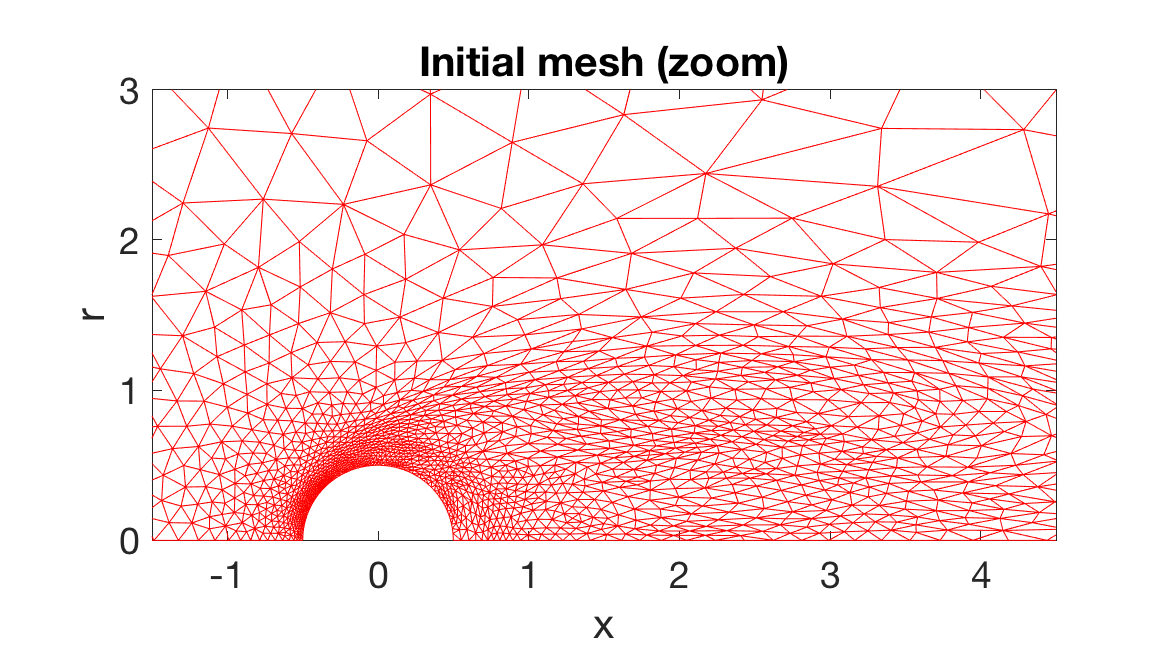
\includegraphics[width=.9 \linewidth]{Cylinder_Mesh.png}
%\vspace{-.5cm}
%\vspace{-.5cm}
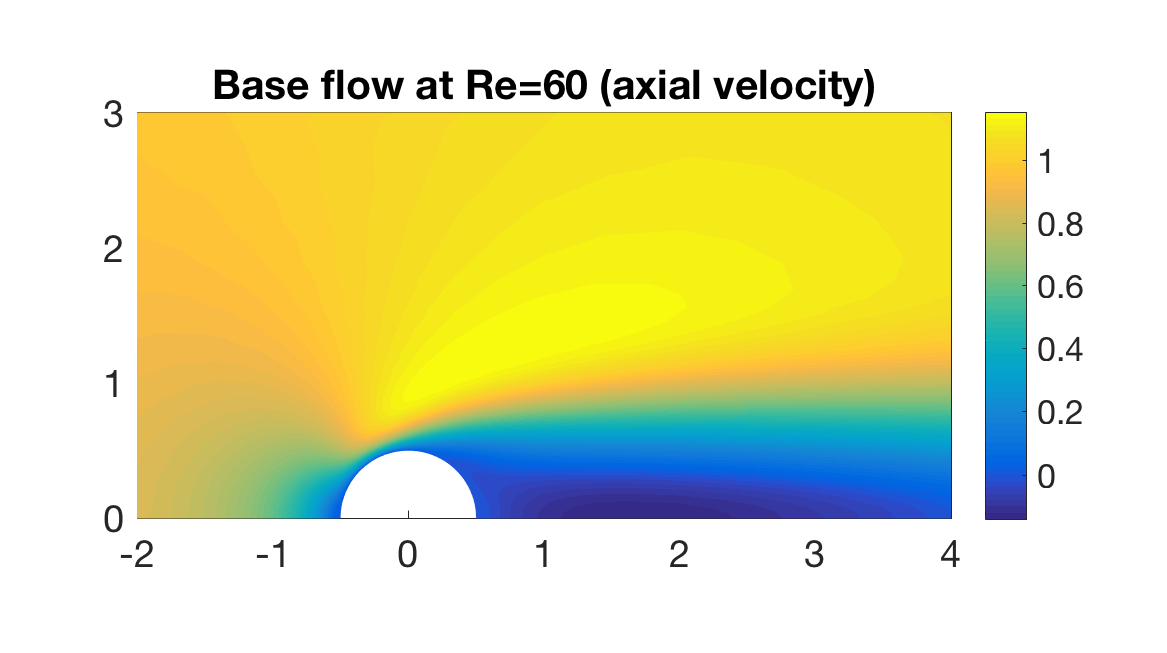
\includegraphics[width=.9 \linewidth]{Cylinder_BaseFlowRe60.png}
%\vspace{-1.cm}
\caption{Base flow (streamwise velocity component) for the flow over a cylinder at $Re=60$.}
\label{fig:Baseflow}
\end{figure}

\begin{figure}
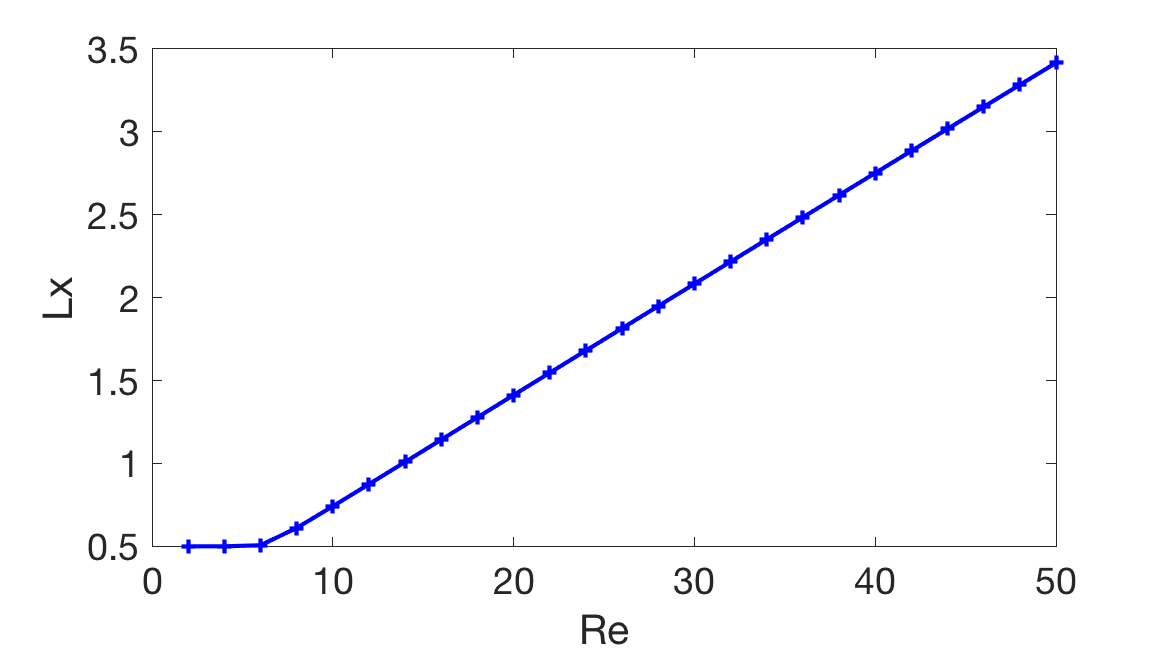
\includegraphics[width=.9 \linewidth]{Cylinder_Lx_baseflow.png}
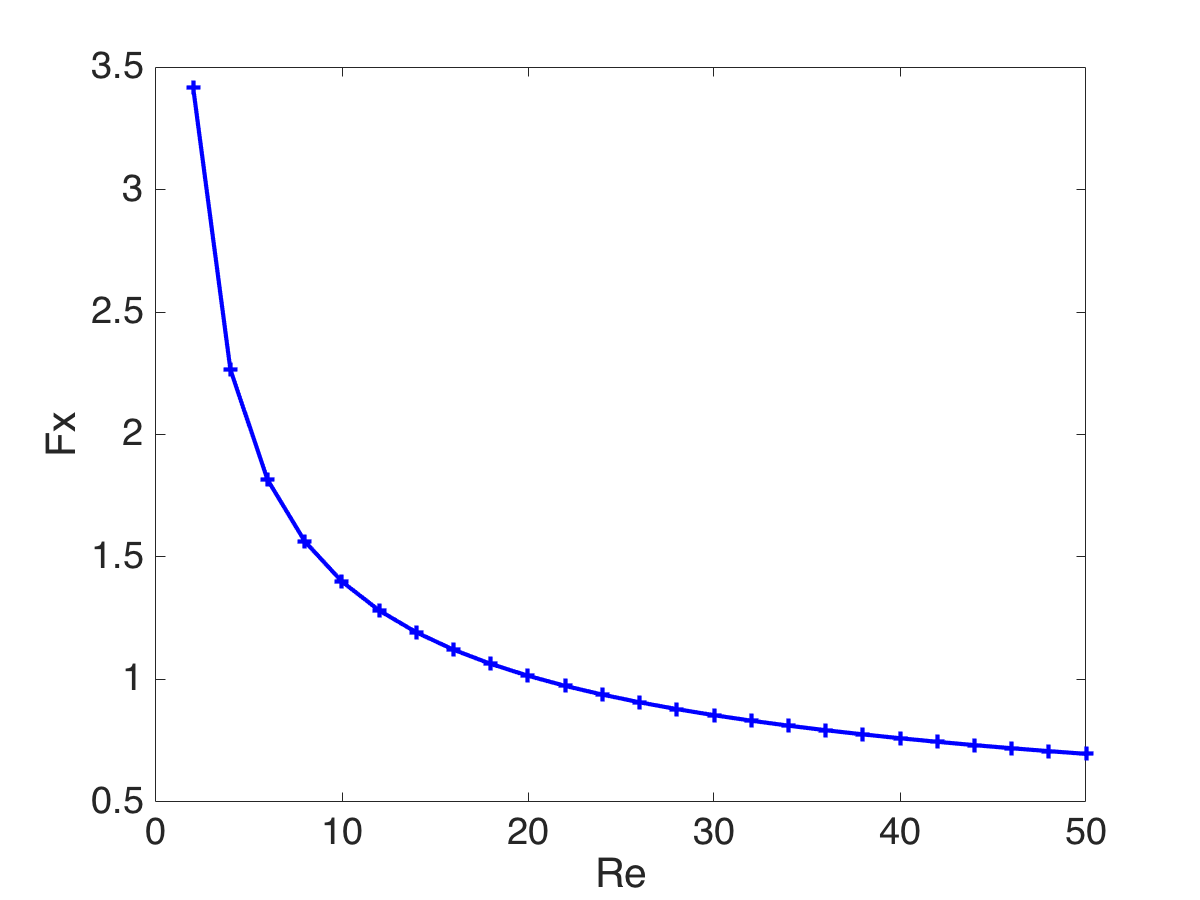
\includegraphics[width=.9 \linewidth]{Cylinder_Fx_baseflow}
\caption{Recirculation length $L_x$ $(a)$  and nondimensional drag $F_x$ ($b$) of the base flow over a cylinder as function of $Re$.}
\label{fig:LxandDrag}
\end{figure}




\subsection{Mesh adaptation procedure}
\vspace{.2cm}

As for any numerical method, a crucial point in the numerical efficiency is the design of the mesh. The finite element method allows to use unstructured mesh and hence to locally adapt the refinement. %Following Sipp \& Lebedev, 
The most common procedure is to decompose the domain into several parts with different grid densities; for instance for the wake of a cylinder, we will design a near-wall region with very small  size, a wake region with intermediate mesh size, and an outer region with large mesh size. The inconvenient is that the design relies on an a priori expectation of the regions where gradients will be large. 

In our implementation, we used an automatic mesh adaptation method. %which provides an optimal mesh adapted to the structure of the flow. 
The implementation relies on the AdaptMesh procedure of the FreeFem++ software. This procedure is detailed in detail in ref. \cite{adapt}. 
In short, the classical Delaunay-Voronoi algorithm produces a mesh with gridpoint distribution specified by a {\em Metric } matrix $\cal M$. The AdaptMesh algorithm consists of using as a metric the {\em Hessian} (second-order spatial derivatives) of an objective function $u_h$ defined over the domain, i.e. ${\cal M} = \nabla \nabla u_h$. The precision can be controlled by specifying an objective value for the interpolation error of the function on the new mesh.

To build an optimal mesh for the base-flow calculation, the idea is to use as the objective function $u_h$ the solution ${\bf u}_b$ itself, as computed on a previous mesh.%The procedure thus ensures that the mesh will be locally adapted to the gradients of the base flow. 
The base flow is then recomputed on the adapted mesh, providing a better approximation of the solution. The procedure can be repeated a few steps to ensure a right convergence.

The mesh generated in the previous way may not be optimal for the stability calculations as the structure of the eigenmode may be more complex than that of the base flow. To remedy with this, the idea is to subsequently adapt the mesh to both the mesh flow and the results of the stability calculation. This is easily done with FreeFem, as the  AdaptMesh procedure can be used with several objective functions. We have experimented three different ideas. The first is to adapt the mesh to the base flow and the structure of the leading eigenmode. The second idea is to use the adjoint mode instead of the direct mode for mesh adaptation.
The third idea is to adapt the mesh to the base flow and the structural sensitivity. This idea is supported by Giannetti \& Luchini\cite{GiannettiLuchini} who showed that the accuracy of the stability results for the flow past a circular cylinder is strictly related to the mesh characteristics in the wavemaker region, i.e. the region where the structural sensitivity reaches its maximum values. 
Results show that the three procedures yield the same values for base flow characteristics and eigenvalues with less than $0,3\%$ deviation, but that compared to the two previous ideas mesh adaptation to structural sensitivity result in a mesh with much less grid vertices, leading to much faster computations (see appendix A). So, if one is interested only in the eigenvalues, for instance to plot growth rates as function of Reynolds or to identify the critical Reynolds number, mesh adaptation to the sensitivity gives the best option. On the other hand, if one is interested in the detailed structure of the eigenmode, which may extend far away from the wavemaker region, it is advised to use mesh adaptation on the eigenmode. 

In our implementation, the whole process is performed using the Matlab driver {\em SF\_AdaptMesh.m} ; the kind of adaptation  (to base flow only, to eigenmode, or to sensitivity) is decided by the the nature of the eigenmode object transmitted to this function.






\section{Illustration for the wake of a cylinder} 
\vspace{.2cm}

\paragraph{Problem description}
Here, we consider the two-dimensional flow of an incompressible fluid of density $\rho$ past a circular cylinder. 
All flow quantities are normalized using the uniform incoming velocity $U_{\infty}$ and the cylinder diameter $D$, 
which are the characteristic velocity and length scales used for the definition of Reynolds number $Re= U_{\infty} D / \nu$.
The origin of the cartesian frame of reference is considered located on the cylinder axis, the x-axis is chosen to be parallel to 
the incoming free-stream velocity while the y-axis with the cross-stream velocity. 
The dimensions of the computational domain are the following: $-40 \le x/D \le 80$ and $0 \le y/D \le 40$ (boundary conditions and their implementation are detailed in appendix D).
Note that we take advantage of the symmetry properties of the problem to use a half-domain for resolution. 
%We impose a no-slip condition $(u=0,v=0)$ on the cylinder surface (${\Gamma_{cil}}$), a uniform velocity $(u=1,v=0)$ at the inflow 
%$x/D=-40$ and a no-stress condition at the outlet $x/D=80$ and on the lateral boundaries of the computational domain $y/D=\pm 40$.

%Domain dimension $[-40,80]x[0,40]$. No-stress conditions at outlet AND LATERAL BOUNDARY.
The hydrodynamic loads can be obtained by integrating the stress tensor over the cylinder surface.
In particular, the hydrodynamic lift and drag forces read
\footnote{ Remark that $F_x$ and $F_y$ are actually nondimensional forces per unit length. 
For a cylinder of diameter $D$ and length $L$ (assuming $L\gg D$ so that the assumption of 2D flow makes sense), 
the corresponding dimensional forces are $F_x^* = \rho U_\infty^2 D L F_x $ and $F_y^* = \rho U_\infty^2 D L F_y$. 
Alternatively, one may characterize the forces through the drag and lift coefficients $C_x$ and $C_y$. With the usual convention, 
The connection between the nondimensional forces and the force coefficients is $C_x = 2 F_x$ ; $Cy = 2 F_y$.
}
\be{drag}
F_x = {\cal D}_{Re} ({\bf u},p) \equiv 
  \int_{\Gamma_{cyl}} \left[-p {\bf n} + \frac{2}{Re} {\mathsf{D}}({\bf u}) \cdot {\bf n} \right]   \cdot {\bf e_x} d\ell,
\ee
\be{lift}
F_y = {\cal L}_{Re} ({\bf u},p) \equiv
  \int_{\Gamma_{cyl}} \left[-p {\bf n} + \frac{2}{Re} {\mathsf{D}}({\bf u}) \cdot {\bf n} \right]   \cdot {\bf e_y} d\ell. 
\ee
where $\Gamma_{cyl}$ is the boundary of the cylinder. %The factor 2 stands for the fact that our numerical domain is half the physical domain.


\paragraph{Mesh adaptation procedure}

Let us consider now the matlab code reported in figure \ref{Listing2}. First we build an initial mesh (line 1), and compute base flow solutions for increasing values of the Reynolds number up to $Re = 60$ (lines 3-9).
Then we perform the mesh adaptation with the structural sensitivity, as explained previously (line 13). 
The resulting mesh, depicted in figure \ref{fig:mesh2}, is used for the rest of the computations presented in this paper (except for computing
the energy of the nonlinear perturbation displayed in figure \ref{fig:HB_SC_DATA_COMP}$(d)$ which requires a heavier mesh). 
Appendix A presents additional test regarding mesh convergence, and demonstrate that results obtained with the resulting mesh are trustable within $0.3\%$ accuracy for the eigenvalue. It must be emphasized  that the mesh generated through this adaptation process is very light, with only 2048 vertices, which is significantly less than reported in previous work (for instance, in their mesh convergence studies, \cite{SippLebedev} and \cite{MLugo2014} used respectively 190868  and 6731 vertices).


%It is shown that as well as doing mesh adaptation with the eigenmode structure instead of the sensitivity, as discussed above, gives comparable results within $1\%$ as for the eigenvalue of the most amplified mode.







%The produced outputs (lines 14-17) gives information about the resulting mesh. 
%Note the values $h_{min}$ and $h_{max}$ of the smaller and larger edges, as well as the local grid size at four points A,B,C,D defined as $(x_A,y_A) = (0.5,0)$ (at the surface of the cylinder at the position of maximum shear), $(x_B,y_B) = (0.5,2.5)$ (at the location of the peak of structural sensitivity, see next section), $(x_C,y_C) = (0.,4)$ (in the near wake), and $(x_D,y_D) = (0.,10)$ (in the the far wake). Finally, the base flow is automatically recomputed on the resulting mesh (line 18-19). Finally, lines 21-22 plot the mesh and base flow structure, producing the result displayed in figure (\ref{fig:Baseflow}).

\paragraph{Base flow}

Having thus produced a convenient mesh, we can now illustrate the properties of the base flow as function of Reynolds number. Figure \ref{Listing2} shows how to compute and plot with StabFem the two most commonly studied quantities, namely the recirculation length $Lx(Re)$, i.e. the location of the stagnation point at the rear of the recirculation region, and the drag force $F_x(Re)$.
Note that the object \verb|bf| is defined as a structure with fields \verb|Fx| and \verb|Lx|. 
The resulting plots are given in figure \ref{fig:LxandDrag}, and are in good agreement with known results for this classical problem.
In particular, for low Reynolds, the recirculation $L_x(Re)$ is equal to $0.5$ (which is the radius of the cylinder) indicating the absence of a recirculation region. The latter appears for $Re > 4.8$, in accordance with known results.

An illustration of the structure of the base flow is given in figure \ref{fig:Baseflow},  for the case $Re = 60$. The contour line on this plot corresponds to the iso-level $u_x = 0$, and allows to visualize the recirculation region associated to this base flow. In accordance with figure \ref{fig:LxandDrag}$(b)$, for $Re = 60$ the recirculation length is $L_x = \approx 4.07$.




%\subsection{Implementation}

%\subsection{Application to the cylinder}


%\clearpage

%We now review the main concepts of linear stability approach and explain how such calculations are implemented in our software.

\begin{figure}
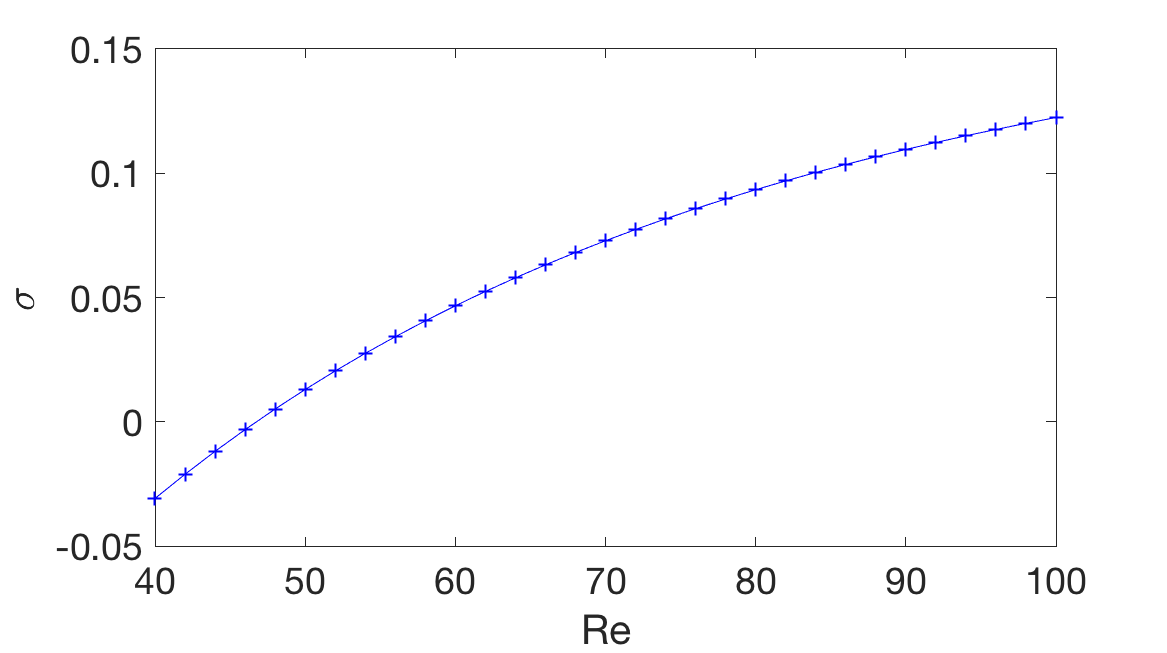
\includegraphics[width=.9 \linewidth]{Cylinder_Sigma_Re.png}
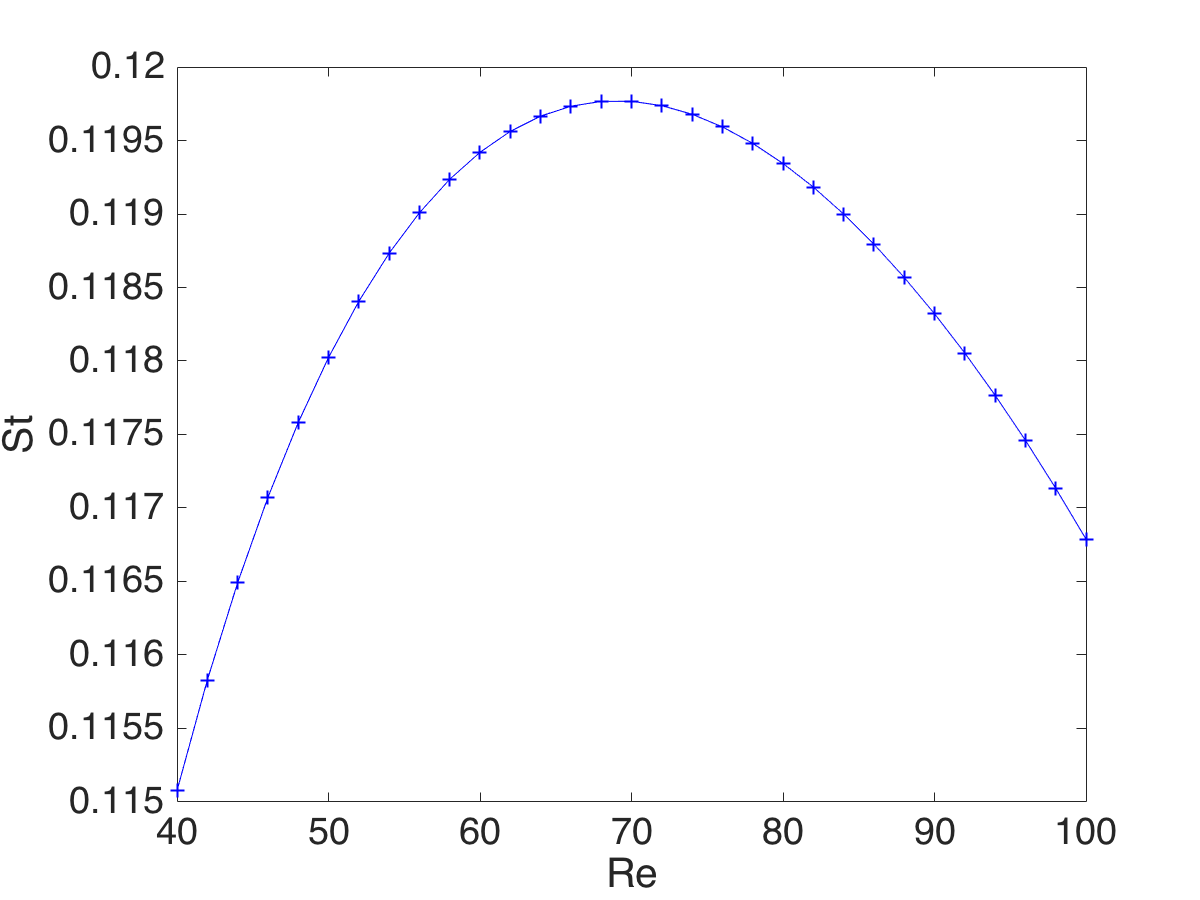
\includegraphics[width=.9 \linewidth]{Cylinder_Strouhal_Re.png}
\caption{Growth rate $\sigma$ $(a)$  and Strouhal number $St = \omega/2\pi$ ($b$) as function of Reynolds number}
\label{fig:SigmaOmega}
\end{figure}

\begin{figure}
%\vspace{-.5cm}
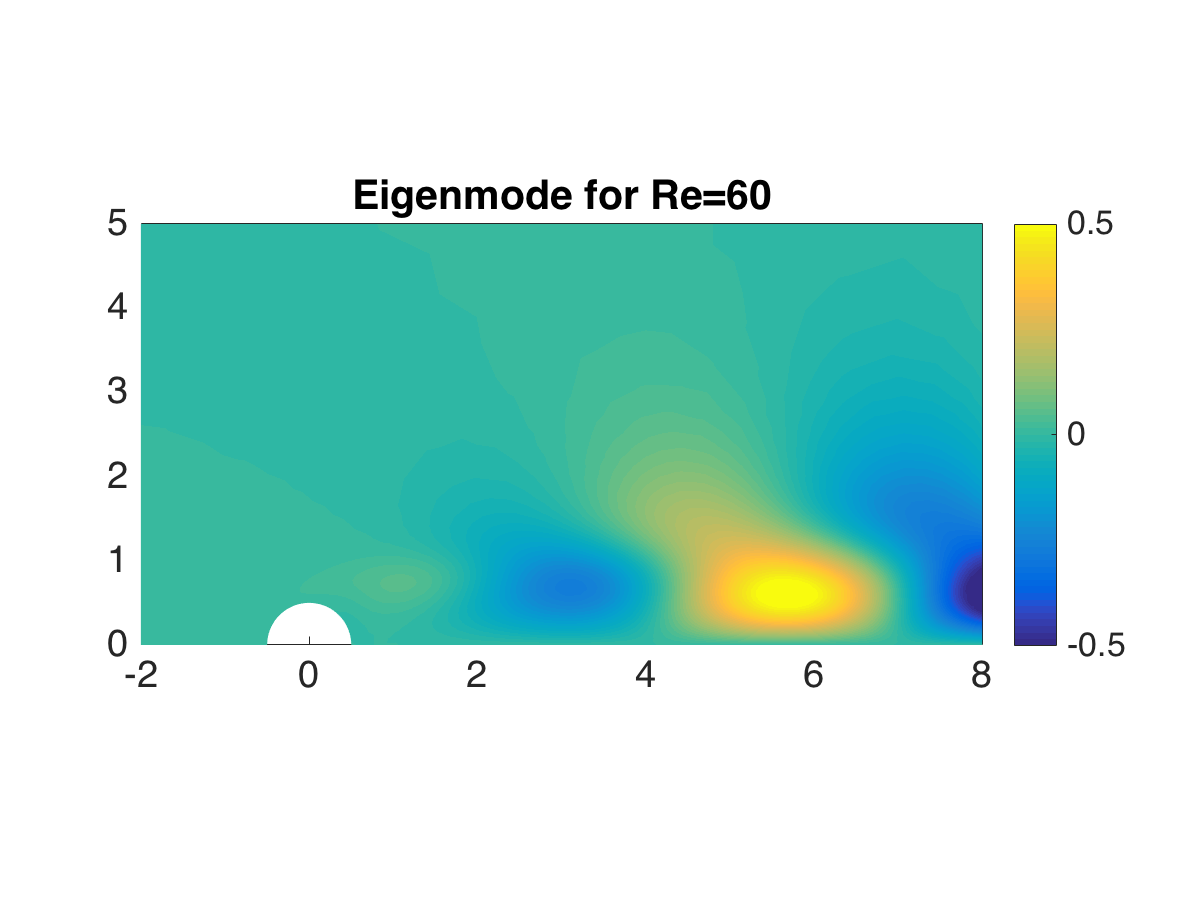
\includegraphics[width=.9 \linewidth]{Cylinder_EigenModeRe60_AdaptD.png}
%\vspace{-.5cm}
%\vspace{-.5cm}
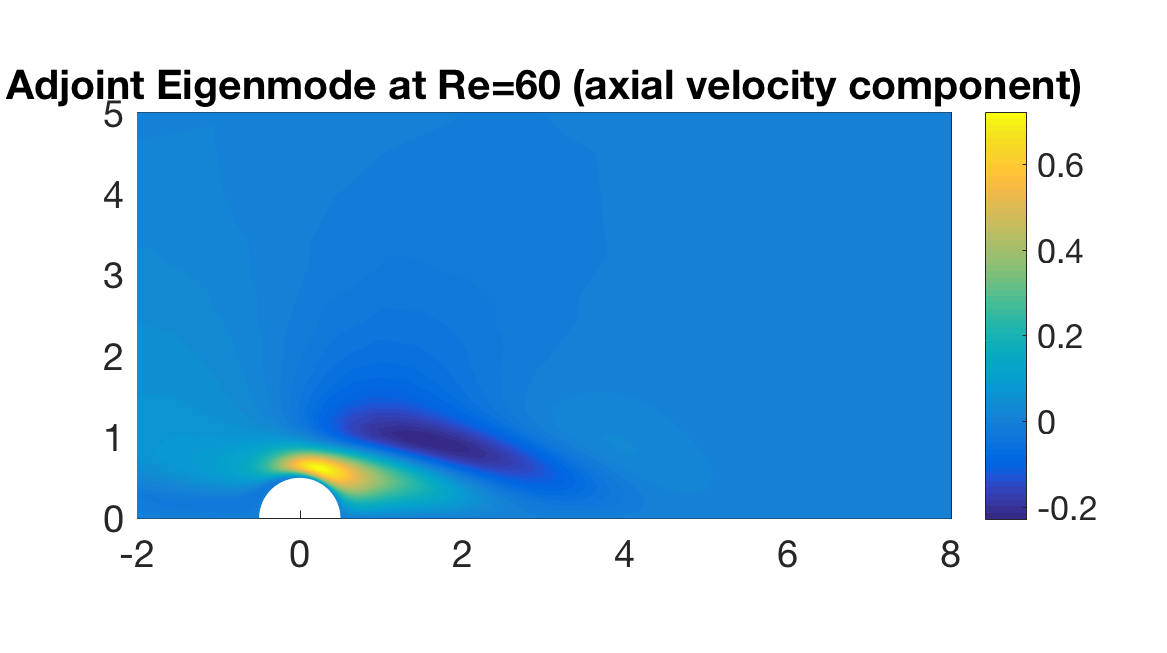
\includegraphics[width=.9 \linewidth]{Cylinder_EigenModeAdjRe60.png}
%\vspace{-.5cm}\vspace{-.5cm}
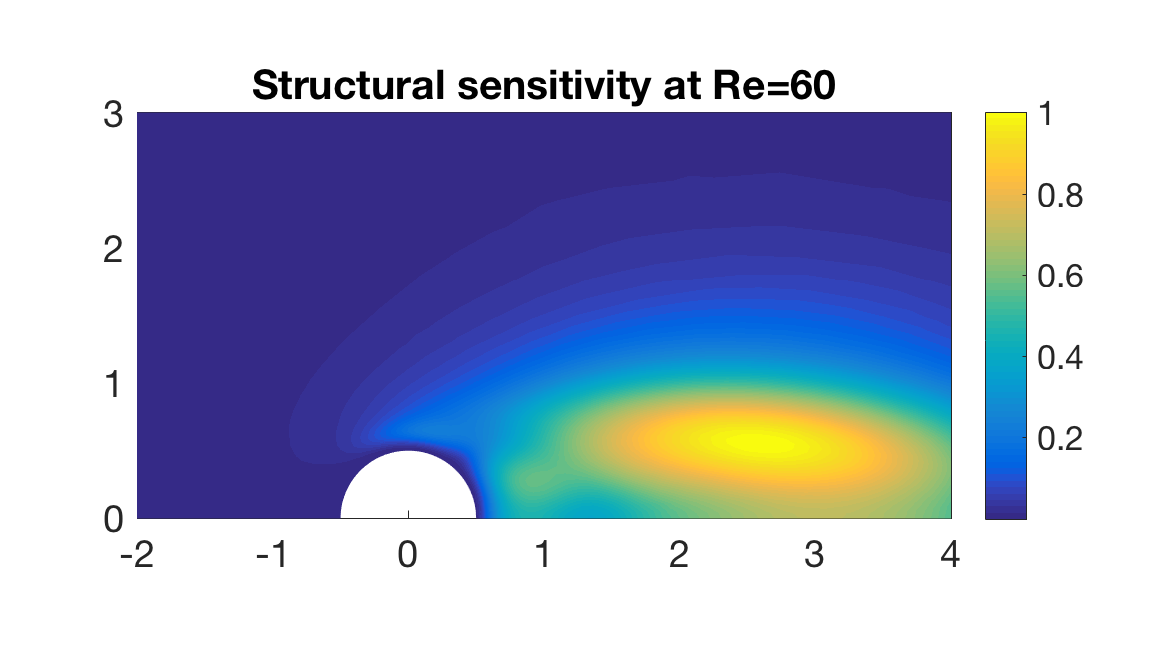
\includegraphics[width=.9 \linewidth]{Cylinder_SensitivityRe60.png}
%\vspace{-.5cm}
\caption{Contour plot of the streamwise velocity component: $(a)$ (Direct) Eigenmode; $(b)$ Adjoint mode and ($c$) Structural sensitivity field for the cylinder's wake at $Re=Re_c = 46.7$.}
\label{fig:Eigenmode}
\end{figure}


%\begin{figure*}
%\small
%\begin{lstlisting}
%\end{lstlisting}
%\normalsize
%\caption{Illustration of the procedure to compute stability properties and adapt the mesh using StabFem (from script {\em SCRIPT\_CYLINDER.m}. }
%\label{listing4}
%\end{figure*}

\paragraph{Linear stability results}

We investigate the stability of the base flow fields by performing a parametric study of the eigenproblem 
(\ref{Eigen_matricial}). In this way, we determine the critical Reynolds number $Re_c$ at with the steady base flow
first becomes unstable: to this end it is useful to remember that a flow state is 
linearly unstable when the real part of 
the leading eigenvalue, i.e. the growth rate, is positive. 
Figure \ref{fig:SigmaOmega} shows growth rate and the Strouhal number 
$St=a\omega/2 \pi U_{\infty}$ as a function of the 
Reynolds number. It is easy to check that the critical Reynolds number is about 47 
for the first mode. 
The associated direct eigenmode is depicted in figure \ref{fig:Eigenmode}. The 
spatial structure of this mode 
extends downstream of the bluff body and is characterized by streamwise 
extended spatial disturbances. 
On the other hand, the adjoint mode is highly localized near the cylinder 
on the upper (and lower) side of the body surface. 
We recall that the adjoint field provides useful information about the mechanism to
flow receptivity to momentum forcing and mass injection.
We note also that this receptivity decays rapidly both upstream and downstream 
of the bluff body.

The structural sensitivity field displayed in figure \ref{fig:Eigenmode}c)
is obtained by evaluating eq. \ref{Structursens}.
In particular, we plot the spectral norm of the sensitivity tensor, it 
gives the maximum possible coupling among the velocity components. 
This spatial map can be used to identify the flow region where the 
instability mechanism acts.


\section{Nonlinear global stability approaches}
\vspace{.2cm}
%\section{Computing the limit cycle for $Re>Re_c$ with Harmonic Balance}


%For $Re\right>Re_c$, the linear stability analysis based on the {\em base flow} does not allow to predict the properties of the limit cycle; in particular the Strouhal number is substantially underestimated. %It has been shown that investigating the stability properties of the {\em mean flow} obtained by averaging time-marching solution gives a better accordance. Attempts to on a rigourous basis  

In the past decade, efforts have been devoted to extend the range of validity of global approaches into the nonlinear regime for $Re>Re_c$, with the double objective to describe the properties of the limit cycle reached after saturation and to derive amplitude equations describing the transitent dynamics towards this cycle. The two main milestones in this direction  are the {\em weakly nonlinear model}  (WNL) of Sipp \& Lebedev \cite{SippLebedev} and the {\em self-consistent model} (SC) of Manti\v{c}-Lugo et al \cite{MLugo2014}.
 In this review, we will address only the first of the two questions, namely  the description of the saturated cycle, and leave aside the question of transient dynamics. We will successively review the two aforementioned models, in a simplified formulation devoted to describe only the saturated cycle. We also provide a simple implementation of these two models. Finally, in line with the previous section, we will again illustrate with results obtained for the wake of a cylinder.
  
 In this part, to simplify the notations, we symbolically write the Navier-Stokes equations as $\partial_t {\bf u} = {\cal NS} ({\bf u})$, therefore dropping the systematic reference to the incompressibility constraint and associated pressure field. The same is done with the linearized operator ${\cal LNS}_{{\bf U}}( {\bf u})$. 

\subsection{General definitions in the nonlinear regime}



In the nonlinear regime, the {\em base flow} introduced in the linear theory is no longer relevant, especially when the oscillation amplitudes become large. 
Instead, one may define a {\em mean flow} by time-averaging : 
%{\color{red} we taken the Reynolds decomposition ${\bf u}={\bf u}_m({\bf x})+{\bf u}'({\bf x},t)$, with ${\bf u}'$ the nonlinear perturbation and ${\bf u}_m$ the {\em mean flow} defined as the time-average  of the flow:}

\be{defumean}
{\bf u}_m({\bf x})  = \frac{1}{T} \int_0^{T}  {\bf u}({\bf x},t)  dt,
\ee
where $T = 2\pi/\omega$  is the period of the oscillation cycle. The difference between the instantaneous solution and the mean flow is then called the {\em nonlinear perturbation}, defined as 

\be{defuprime}
{\bf u}'({\bf x},t) =   {\bf u}({\bf x},t)-  {\bf u}_m({\bf x}).
\ee

A convenient measure of the unsteady part of the flow, which has been adopted in both the WNL and SC models, is the energy-amplitude, defined as the square-root of the total energy associated to the nonlinear perturbation:
\be{defAnergy}
A_E = \sqrt{\frac{1}{T} \int_0^{T} \left( \int_\Omega | {\bf u}' |^2 \, dS \right) dt}.
\ee

In the next sections we will document the predictions of the WNL and SC models regarding the quantities $A_E$ and $L_x$ adopted in past studies. In addition, we will document two other quantities of practical interest : the Drag and Lift forces $F_x$ and $F_y$ exerted on the cylinder. 
Both are periodic functions of time and; owing to symmetry consideration, the drag contains only even harmonics and the lift only odd harmonics:

%\be{drag_lift_def}
%\begin{cases}
%F_x=F_{x,0} + \sum_{n=1}^\infty \big( F_{x,2n,c} \cos ( 2 n \omega t) + F_{x,2n,s} \sin( 2 n  \omega t ) \big) \\
%\begin{split}
%F_y  =  \sum_{n=1}^\infty \big(  F_{y,{2n-1},c} \cos ((2n-1) \omega t ) +\\
% F_{y,(2n-1),s} \sin ((2n-1) \omega t) \big)
%\end{split}
%\end{cases}.
%\ee
\begin{align}
F_x &=F_{x,0} + \sum_{n=1}^\infty \big( F_{x,2n,c} \cos ( 2 n \omega t) + F_{x,2n,s} \sin( 2 n  \omega t ) \big),
\\
\begin{split}
F_y  & =\sum_{n=1}^\infty \big( F_{y,{2n-1},c} \cos ((2n-1) \omega t )\\
             &\qquad + F_{y,(2n-1),s}  \sin ((2n-1) \omega t) \big).
\end{split}
\label{drag_lift_def}
\end{align}



In the sequel we will focus on the {\em mean drag}  $F_{x,0}$ and on the fundamental components of the lift  
$F_{y,1,c}$ and $F_{y,1,s}$. These quantities are easily extractible from a numerical simulation or an experiment, and we will
show how they can be predicted from the nonlinear global approaches.
 
  

   
%MThe mean drag is given by 

%$$F_{x,m} = D(u_m)$$
%with "Drag" operator defined in equation ().

%The oscillating lift $F_y(t)$  is a	 periodic function of period $T$, and we will 
%$$F_y = F_y,c


%The first milestone in this direction is the work of Sipp \& Lebedev \cite{SippLebedev} who used a weakly nonlinear development in terms of the distance to the threshold $Re-Re_c$. However, although derived on rigorous grounds, the weakly nonlinear development has a very limited range of validity and already fails for $(Re-Re_c) \approx 1$.
%More recently,  Manti\v{c}-Lugo et al \cite{MLugo2014} proposed an alternative approach termed {\em Self-consistent model} which succeeds in predicting the dynamics up to $Re =120$ and more. 
%This model was build as a linear stability approach build on a {\em mean flow} which includes a retroaction of the eigenmode. However, if one is interested in the limit cycle and not the transient,
%the approach is actually equivalent to a Fourier series decomposition of the flow with respect to time (an approach also known as {\em harmonic balance}) retaining only the two first terms. 
%The approach is based on a generalisation of the eigenmode ansatz \ref{} and 

%In the next sections, we thus successively present the weakly nonlinear model, the self-consistent model, and propose a direct resolution method for this latter model. 


%The relation with the initial method of Mantic-Lugo et al. will be discussed afterwards.

\subsection{The weakly nonlinear model}

%\paragraph{Analysis}


\begin{figure*}
\small
\lstinputlisting{Script_Cylinder_Part2.m}
 \normalsize
\caption{Illustration of the procedure for nonlinear calculations using StabFem (extract from script {{\em SCRIPT\_CYLINDER\_ALLFIGURES.m})}. }
\label{fig:listingNL}
\end{figure*}



We first review the weakly nonlinear model of Sipp \& 
Lebedev\cite{SippLebedev}, also discussed by Gallaire et al. \cite{FDR2016}.  
The initial derivation of \cite{SippLebedev} makes use of a multiple scale method in order to obtained an amplitude equation.
This complete analysis is reproduced in appendix B. In the present paragraph, we give a simplified derivation of this model restricted to the description of the periodic saturated cycle.
The starting point can be taken as the following expansion of the velocity flow field:
\be{WNL1}
\begin{aligned}
&{\bf u} = {}  {\bf u}_{bc} + \epsilon \left[ A_{wnl}  \hat{\bf u} e^{i (\omega_c+\epsilon^2 \omega_\epsilon)  t} + c.c. \right]\\
&+ \epsilon^2 \left[ {\bf u}_\epsilon + |A_{wnl}|^2  {\bf u}_{2,0} + \left(  A_{wnl}^2 {\bf u}_{2,2} e^{2 i(\omega_c+\epsilon^2 \omega_\epsilon)  t} + c.c. \right) \right]\\
& + {\cal O}( \epsilon ^3),
\end{aligned}
\ee



This expansion is built as an asymptotic expansion in terms of the small parameter $\epsilon = \sqrt{1/Re_c - 1/Re}$ corresponding to the distance to the critical Reynolds. 
The zero-order term ${\bf u}_{bc}$ is the base flow at the threshold $Re_c$.

In the first-order term, $\hat{\bf u}$ is the neutral eigenmode at $Re_c$ conveniently normalized (see discussion in appendix B), 
$A_{wnl}$ an amplitude which can be assumed as real, $\omega_c$ the frequency predicted by the linear approach at $Re=Re_c$ and $\omega_\epsilon$ a small deviation of the frequency. 

The second-order term contains three contributions: ${\bf u}_{\epsilon}$ is the modification to the base flow related to the 
increase of $Re$, ${\bf u}_{2,0}$  represents the nonlinear interaction of $\hat{\bf u}$ with its conjugate, ${\bf u}_{2,2}$ the nonlinear 
interaction of $\hat{\bf u}$ with itself. These three terms are computed as solutions of nonsingular linear systems 
(see eqs. \ref{eq:LL1}, \ref{eq:LL2}, \ref{eq:LL3} in appendix B).

At ${\cal O}( \epsilon ^3)$, compatibility conditions have to be imposed to ensure that the problem is correctly posed. These conditions lead to an {\em amplitude equation} which relates the amplitude $ A_{wnl}$ to three parameters $\Lambda, \nu_{0}$ and $\nu_{2}$ which depend
uniquely on ${\bf u}_\epsilon$, ${\bf u}_{2,0}$ and ${\bf u}_{2,2}$, respectively (see equations \ref{LAMBDA}, \ref{NU0} and \ref{NU2} in appendix B). Restricting to the description of the limit cycle, the {\em amplitude equation} takes the form :

\be{WNL3}
i \omega_\epsilon A_{wnl} = \Lambda A_{wnl} - (\nu_0+\nu_2)  |A_{wnl}|^2 A_{wnl}.
\ee


%where the coefficients $\Lambda$, $\nu_0$ and $\nu_2$ are given by We note that $\Lambda$ does not depend on the normalization choice of the eigenmode, discussed later, while $\nu_0$ and $\nu_2$ depend. 
The amplitude $A_{wnl}$ and the correction to the frequency are then determined by considering the real and imaginary parts of this equation, leading to
%\be{AWNL}
$
A_{wnl}= \sqrt{ \frac{\Lambda_r}{\nu_{0,r}+\nu_{2,r}}}
$ and
%\ee
%\be{omegaeps}
$
\omega_\epsilon = \Lambda_i- \Lambda_r \frac{\nu_{0,i}+\nu_{2,i}}{\nu_{0,r}+\nu_{2,r}} 
$
%\ee
where the subscripts $r$ and $i$ represent the real and imaginary parts.
Reintroducing the scaling, the  amplitude $A =  \epsilon A_{wnl} $ and the frequency $\omega$ of the limit cycle are thus predicted as
\be{ANL} 
A =  \epsilon A_{wnl} =\sqrt{ \frac{\Lambda_r}{\nu_{0,r}+\nu_{2,r} }} \sqrt{\frac{1}{Re_c}-\frac{1}{Re}},
\ee
\be{omegaWNL} 
\omega \equiv \omega^{(wnl)} =\omega_c+ \left( \Lambda_i- \Lambda_r \frac{\nu_{0,i}+\nu_{2,i}}{\nu_{0,r}+\nu_{2,r}} \right) \left(\frac{1}{Re_c}-\frac{1}{Re}\right)
\ee 


Finally, as specified above, we explain how the mean drag $F_{x,0}$ and fundamental components $(F_{y,1,c},F_{y,1,s})$ of the oscillating lift can be predicted from the WNL approach.
The mean drag  can be obtained by $F_{x,0} = {\cal D}_{Re}({\bf u}_m,p_m)$, where ${\cal D}$ is the drag operator defined in \ref{drag} and 
$[{\bf u}_m,p_m]$ is the {\em mean flow}  
which corresponds to the time-average of expansion  \ref{WNL1}, namely :
$
[{\bf u}_m,p_m] = [{\bf u}_{bc},p_{bc}] +\epsilon^2 \left( [{\bf u}_\epsilon,p_\epsilon] + A_{wnl}^2 [{\bf u}_{2,0}, p_{2,0} ] \right).
$
Developing the terms as an asymptotic expansion leads to :
\be{drag_cos}
 F_{x,0}(Re) \approx F_{x,0,{Re_c}} +  F_{x,0,\epsilon} \left(\frac{1}{Re_c}-\frac{1}{Re}\right)
\ee 
\begin{equation*}
\begin{aligned}
& \mbox{with} \quad F_{x0,{Re_c}}  = {\cal D}_{Re_c} ({\bf u}_{bc},p_{bc}), \quad \mbox{and}  
\\ 
& F_{x0,\epsilon} = {\cal D}_{Re_c} ({\bf u}_\epsilon, p_\epsilon ) - {\cal D}_{1} ({\bf u}_{bc},0) 
+ A_{wnl}^2 {\cal D}_{Re_c} ({\bf u}_{2,0},p_{2,0}). 
\end{aligned}
\end{equation*}
%_{\epsilon},p_\epsilon)
%D({\bf u}_{\epsilon})- 2\int_{\Gamma_{cyl}}} \mathbf{D} ({\bf u}_{bc}) \cdot {\bf n}  \cdot {\bf e}_x d \ell \right) 
%\\
%&+|A|^2 D({\bf u}_{2,0})\\
%&+2|A|^2\big(F_{x,r}({\bf u}_{2,2})\cos(2\omega t)
%-F_{x,i}({\bf u}_{2,2})\sin(2\omega t) \big),

Similarly the required components of the lift force are obtained by applying the lift operator ${\cal L}$ defined in \ref{lift} 
to the order-one component of the expansion, leading to :
\be{lift_cos}
F_{y,1,c} - i F_{y,1,s} = 2 A_{wnl} {\cal{L}}_{Re_c}( {\bf \hat{u}},\hat{p} ) \sqrt{\frac{1}{Re_c}-\frac{1}{Re}}.
%|A|_i F_{x,i}({\bf \hat{u}})\sin(\omega t) \big),\\
%\end{aligned}
\ee

%\be{lift_cos}
%\begin{aligned}
%F_{y,WNL} =2\big(|A|_r F_{x,r}({\bf \hat{u}})\cos(\omega t)-
%|A|_i F_{x,i}({\bf \hat{u}})\sin(\omega t) \big),\\
%\end{aligned}
%\ee

%where $F_{x}$ and $F_{y}$ are given by and \ref{lift} (with the associated pressure field implicit), respectively . All terms in these equations can be matched with the interesting ones in \ref{drag_lift_def}: $F_{x,0}$ is the first 4 terms of \ref{drag_cos}; $F_{x,2,c}$, $F_{x,2,s}$ are the fifth and sixth terms of \ref{drag_cos}; $F_{y,1,c}$, $F_{y,1,s}$ are the first and second terms of \ref{lift_cos}. We note that the \textit{sin} term is associated to the phase of the forces in a physical way. }

%\iffalse
%\begin{eqnarray}
%\begin{aligned}
%F_{x,WNL} = F_{x}({\bf q}_{bc})&+\epsilon^2 \big( 
%F_{x}({\bf q}_{\epsilon})- 2\mathsf{D}({\bf u}_{bc}) \big)\\
%&+F_{x}({\bf q}_{2,0})|A|^2\\
%&+2F_{x,r}({\bf q}_{2,2}\cos(2\omega t)+
%2F_{x,i}({\bf q}_{2,2}\sin(2\omega t)
%),\\
%\end{aligned}\\
%F_{y,WNL} = |A|^2 \big[ F_{y}({\bf \hat{q}})e^{i\omega_{LC} t} +c.c. \big],
%\end{eqnarray}
%\fi


\paragraph{Implementation and results for the cylinder}




Lines 1-8 of the script shown in figure \ref{fig:listingNL}, which is extracted from the script 
{\sf SCRIPT\_CYLINDER\_ALLFIGURES.m}, illustrate the sequence of commands to 
perform the weakly nonlinear study for the cylinder wake.
On line 2, we first determine the instability threshold, and the corresponding base flow and eigenmode\footnote{This routine uses Newton iteration to directly compute the base flow, the eigenmode, the frequency and the critical Reynolds. The algorithm is very similar to the one presented for the HB, with an additional unknown (Re) and an additional constraint (normalization of the mode). The interested reader should reconstruct easily the whole procedure from the code provided.}. 
On line 3 we solve the adjoint problem required for some terms in the WNL formulation.
On line 4, we then compute all the terms and coefficients of the WNL model.
Lines 6-8 then processes the results in a way they can be plotted.
%{\color{red}The other lines are explained latter.}
%After that, 
%we construct  vectors to store the frequency and the amplitude of the limit cycle in the 
%range $Re = [47.5-100]$. Note that for the computation at $Re=47.5$, we need a guess 
%for the amplitude, which is deduced from the weakly nonlinear approach on line 9. In 
%the sequel of the loop no guess value is prescribed, hence the solver uses 
%continuation.

%{\color{red} 
%The forces coefficients given by $F_x({\bf u})$ and $F_y({\bf u})$ are then converted in a more traditional form, $C_x=2F_x({\bf u})$ and $C_y=2F_y({\bf u})$.
%}



Figure \ref{fig:HB_SC_DATA_COMP} represent the predictions of the WNL approach regarding the frequency (expressed as a Strouhal number through $St = \omega/2\pi$), mean drag, amplitude of the oscillating lift, and energy-amplitude.
As discussed in \cite{SippLebedev} and \cite{FDR2016},  when compared to DNS results the approach gives good prediction in the immediate vicinity of $Re_c$, but deviation appears very rapidly and disagreement is already large at $Re=48$ (although, as discussed by \cite{FDR2016} and also observed  \cite{Tchoufag2015}, a convenient definition of the $\epsilon$ improves the results). 
 These aspects are justified by the perturbative nature of the WNL approach. The description of the limit cycle can be extended to larger $Re$ with the approach presented next.  

\begin{figure}
\begin{center}
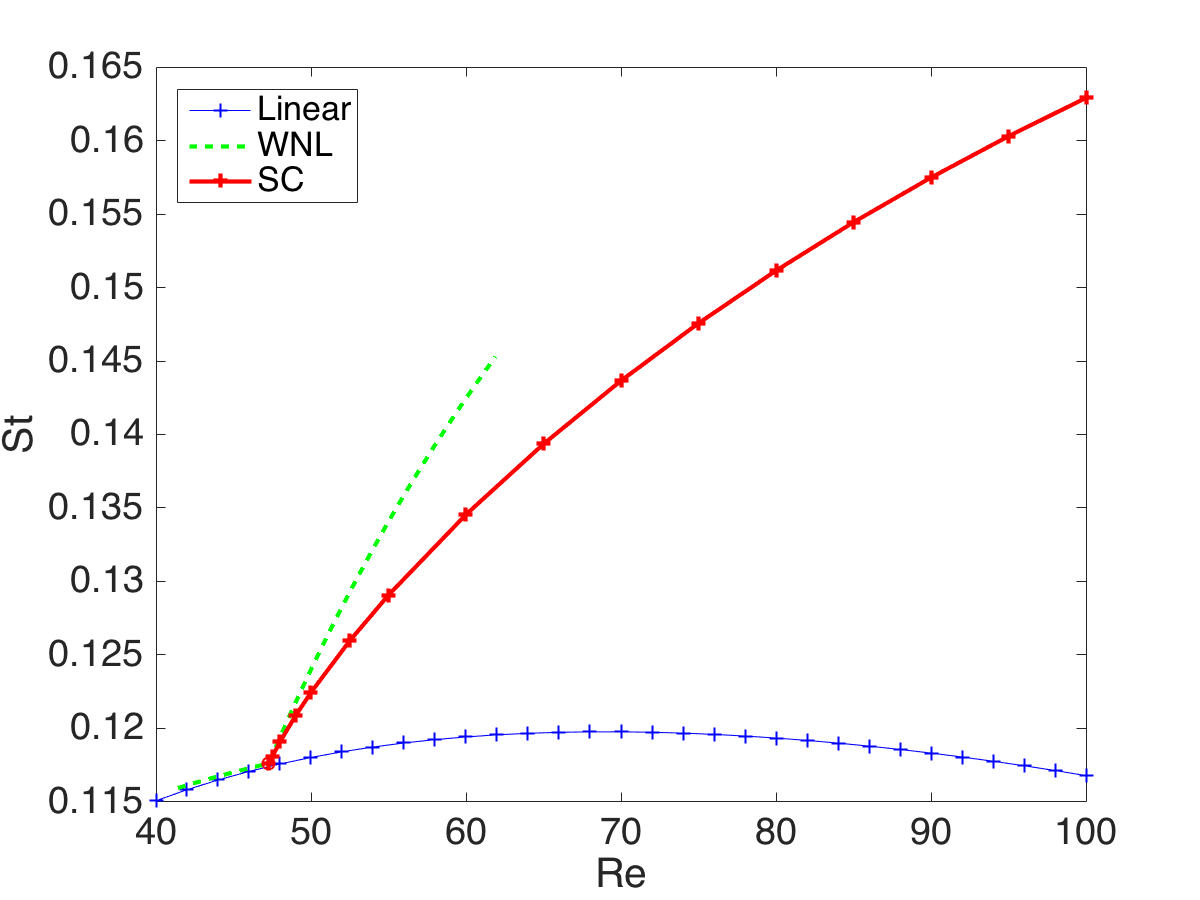
\includegraphics[width=.9 \linewidth]{Cylinder_Strouhal_Re_HB.png}
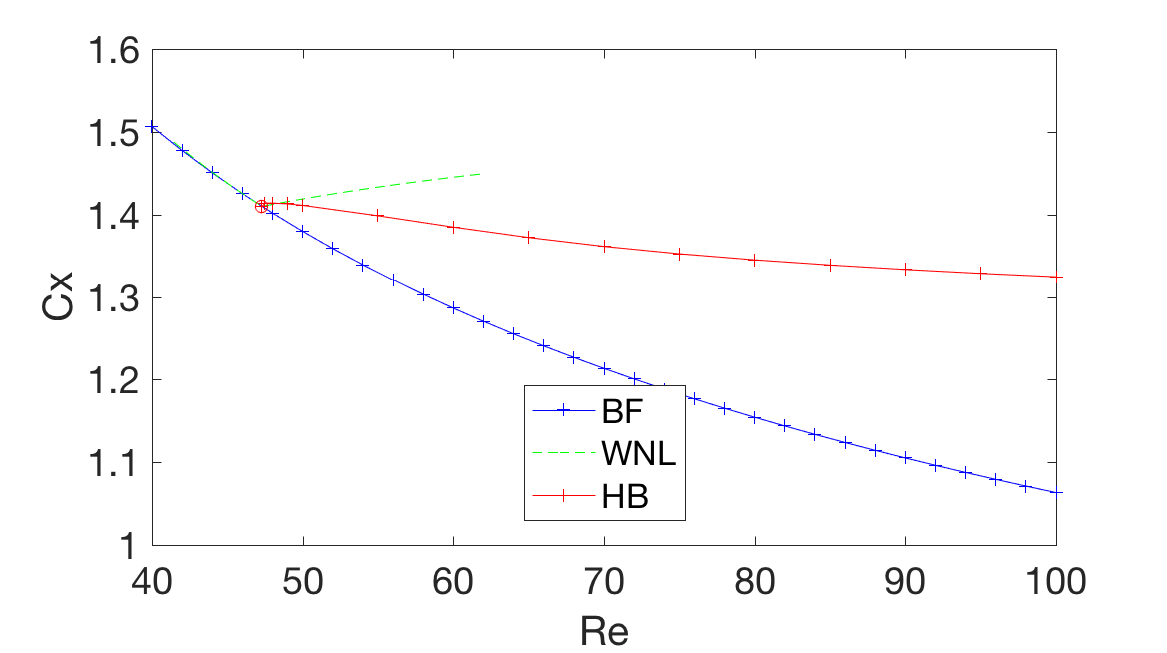
\includegraphics[width=.9 \linewidth]{Cylinder_Cx_Re_HB.png}
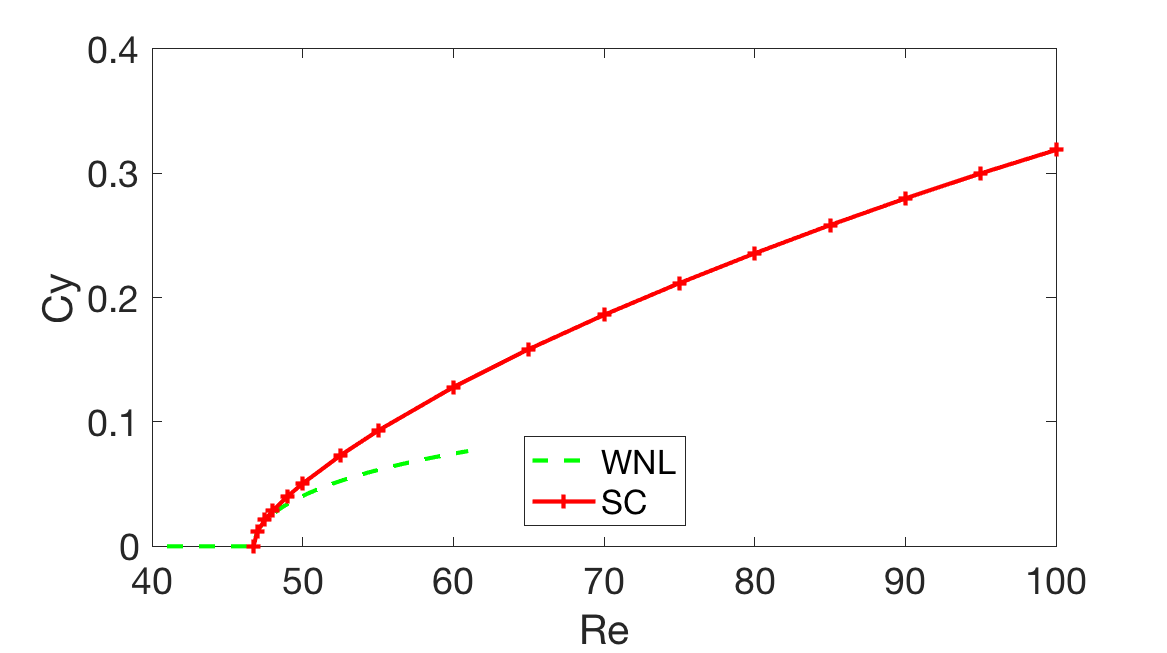
\includegraphics[width=.9 \linewidth]{Cylinder_Cy_Re_SC.png}
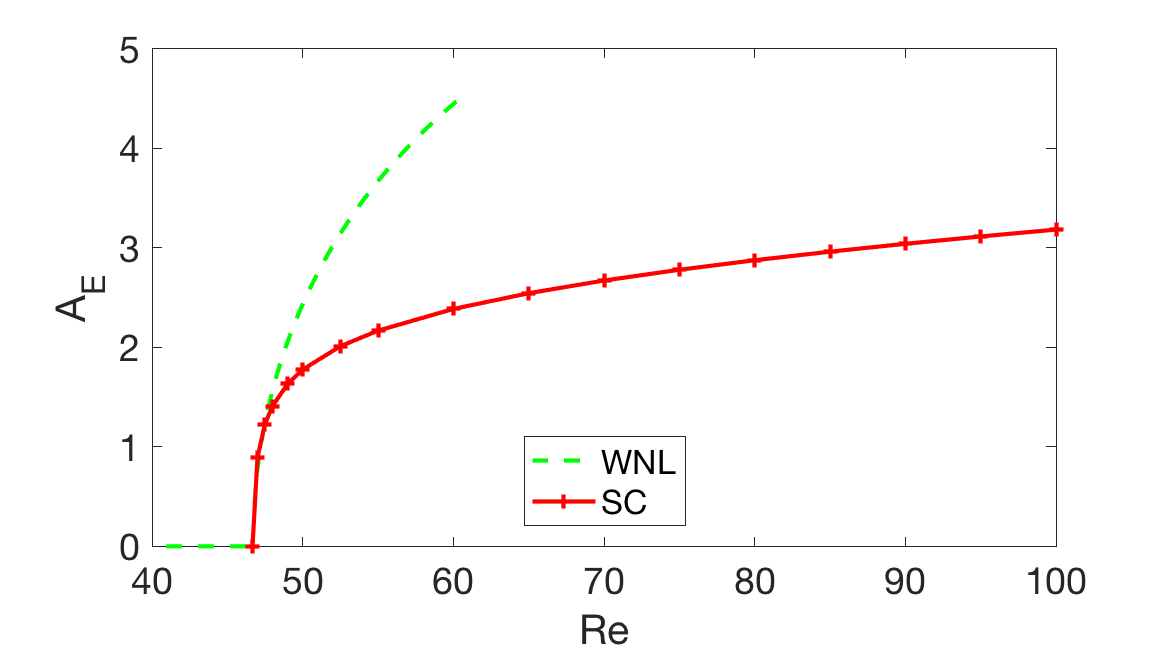
\includegraphics[width=.9 \linewidth]{Cylinder_Energy_Re_SC_AdaptD.png}
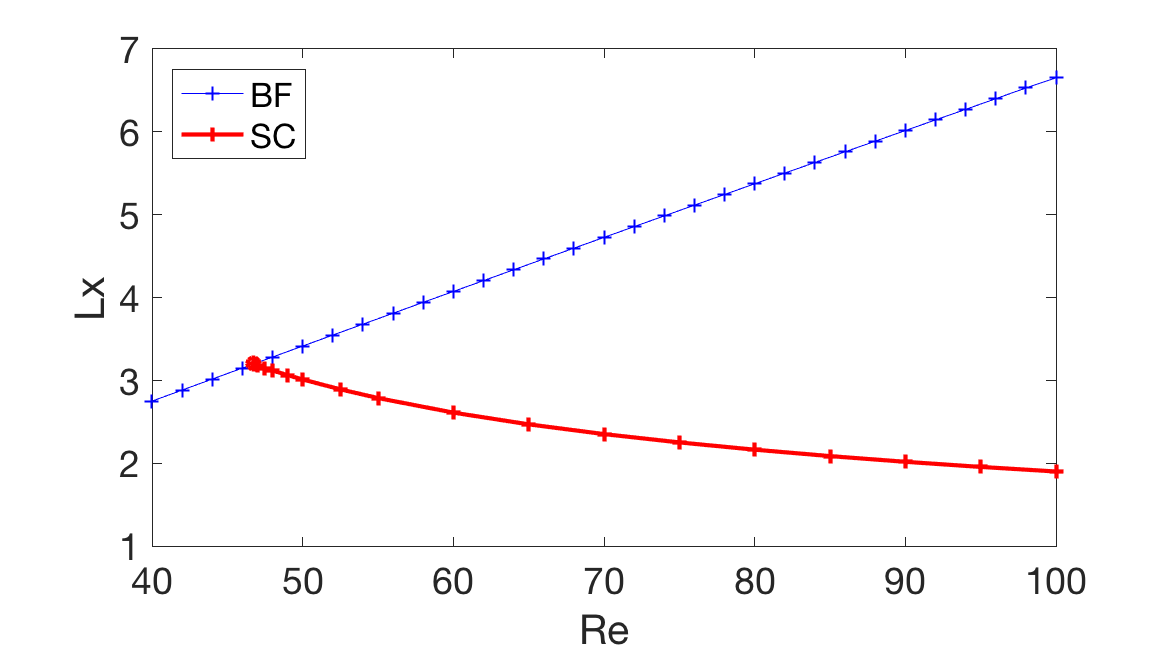
\includegraphics[width=.9 \linewidth]{Cylinder_Lx_Re_HB.png}
\end{center}
\caption{Comparison between the weakly nonlinear results (WNL) the harmonic balance data (HB), and baseflow/linear results : Strouhal number $(a)$, Mean drag $(b)$, amplitude of oscillating lift $(c)$, Energy-amplitude of the nonlinear perturbation $(d)$ and recirculation lenght of mean/base flows ($e)$. 
%c_x should be consistent with the drag definition given at beginning
}
\label{fig:HB_SC_DATA_COMP}
\end{figure}



\subsection{The Self-Consistent model  }
\paragraph{SC model : analysis }

%\begin{figure}
%\begin{center}
%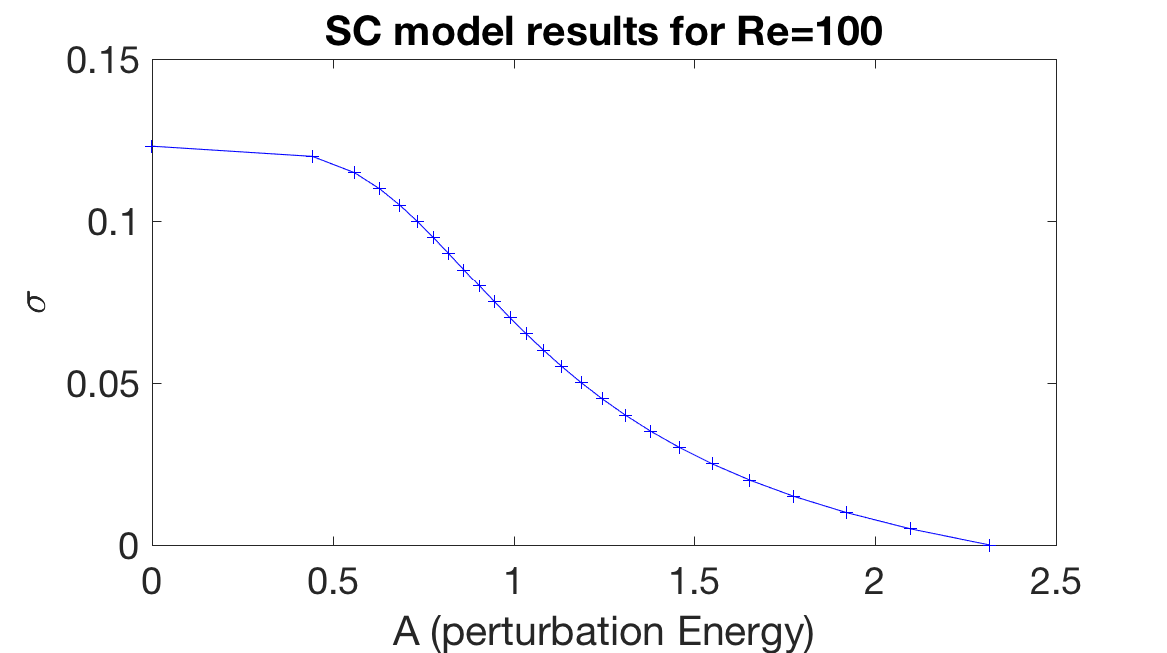
\includegraphics[width=.9 \linewidth]{Cylinder_SC100_EnergySigma.png}
%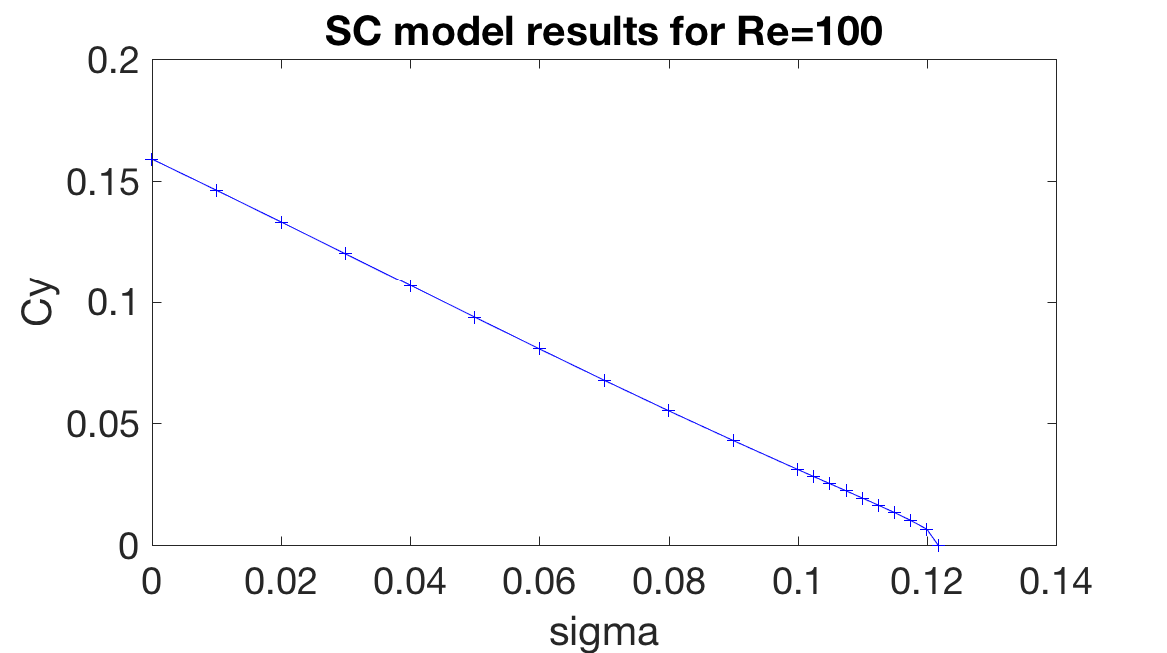
\includegraphics[width=.9 \linewidth]{Cylinder_SC100_CySigma.png}
%\end{center}
%\caption{Self-consistent approach for the wake of a cyrcular cilinder: results at $Re =  100$.}
%\label{fig:SC100}
%\end{figure}


We now briefly review the self-consistent model as introduced by Manti\v{c}-Lugo et 
al \cite{MLugo2014}. In its original exposition, the authors adopted a pseudo-eigenmode expansion of the flow 
as follows: 
\be{SC}
{\bf u } = {\bf u }_m + A_{sc} \left[ \tilde{{\bf u }}_1 e^{\sigma_{sc} t + i \omega_{sc} t} +   \overline{\tilde{\bf u }_1} e^{\sigma_{sc} t  -i \omega_{sc} t} \right],
\ee  
where ${\bf u }_m$ is the {\em mean flow} as previously defined,  $\tilde{{\bf u }}_1$ is a pseudo-eigenvector which is normalized by the condition  $||\tilde{{\bf u }}_1|| = 1/\sqrt{2}$, $\overline{\tilde{{\bf u }}_1}$ is its complex conjugate,
$A_{sc}$ is an amplitude parameter directly related to the energy of the oscillating flow, and $\lambda_{sc} = \sigma_{sc} + i \omega_{sc}$ is a pseudo-eigenvalue which depends upon the parameter $A_{sc}$. 

The original version of the model (discussed with some more details in appendix C) allowed to obtain an amplitude equation predicting the instantaneous growth rate $\sigma$ as function of the amplitude $A_{sc}$. However, if we are simply interested in the properties of the limit cycle, not the transient, we may recast the self-consistent model in a simpler way. 


%Figure \ref{fig:SC100} shows the results of the self-consistent model at Re=100.

%\paragraph{{\color{red}First Order Harmonic balance: equations and procedure} }

%\begin{figure}
%\begin{center}
%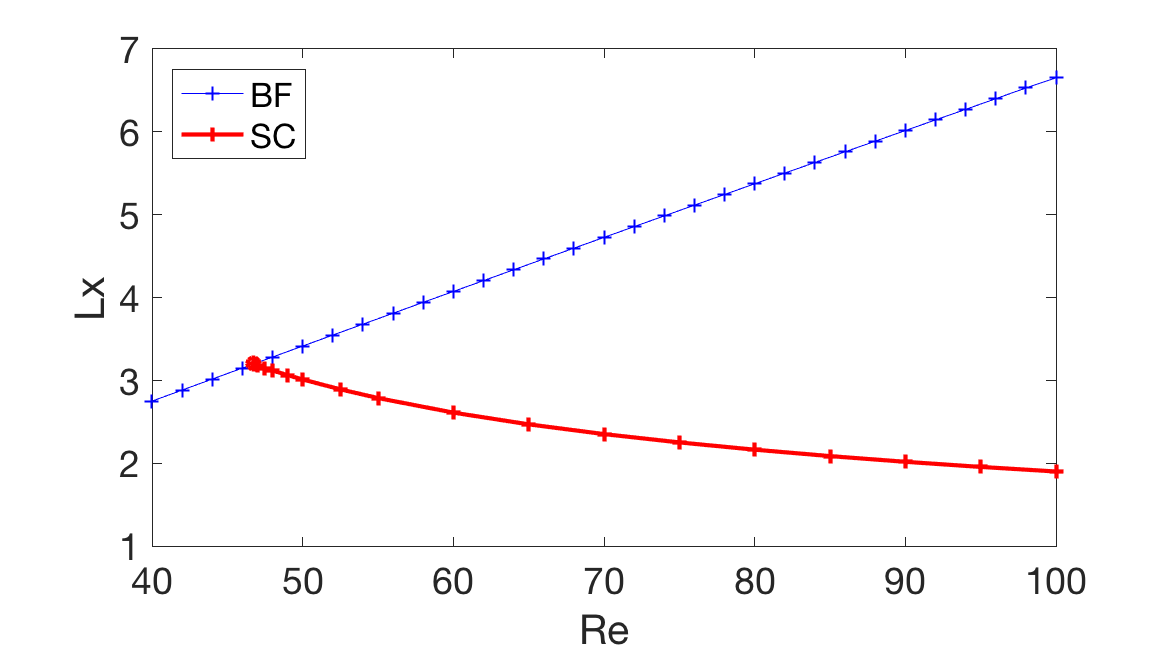
\includegraphics[width=.9 \linewidth]{Cylinder_Lx_Re_HB.png}
%\end{center}
%\caption{Flow past a circular cylinder: length of the wake bubble (measured from the 
%rear stagnation point) for different Reynolds number. Comparison between the base flow bubble and the mean flow bubble computed by using the harmonic balance.}
%\label{fig:recirculation_lengh}
%\end{figure}


%As discussed above, the Self-Consistent model was initially presented by the authors as a rational way to explain the dynamics in terms of a stability analysis of the {\em mean flow}. Furthermore, the resolution method presented by the authors, which involves a double iteration loop, is not easy to implement and not particularly efficient.

%If one is only interested by the properties of the limit cycle and not the transient, the model is actually equivalent to a Fourier series, and amenable to a more direct resolution method. 
We thus start with a truncated Fourier decomposition of the limit cycle under the form:
\be{HB}
{\bf u } = {\bf u }_m + {\bf u }_{1,c} \cos( \omega t ) +   {\bf u }_{1,s} \sin( \omega t ),
\ee
where ${\bf u }_{1,c}$ and ${\bf u }_{1,s}$ are two {\em real} fields describing the nonlinear perturbation at two instants separated by a quarter-period of oscillation, and $\omega$ is the (real) oscillation frequency of the limit cycle (which is not known a priori).  
The connection with the definition of Manti\v{c}-Lugo is as follows :
\be{HBtoSC}
\left( {\bf u }_{1,c} - i {\bf u }_{1,s} \right) = 2 A_{sc} \tilde{{\bf u }}_1.
\ee 

 

Injecting this ansartz into the Navier-Stokes equations and taking the mean value and the first Fourier component leads to the following coupled equations:
\begin{subequations}\label{eq_principal}
\begin{eqnarray}
{\cal NS}(  {\bf u }_m ) = \frac{{\cal C}( {\bf u }_{1,c}, {\bf u }_{1,c}) +{\cal C}( {\bf u }_{1,s}, {\bf u }_{1,s})}{4}, 
\label{HBEq0}
\\
 \omega {\bf u }_{1,s} =  {\cal LNS}_{{\bf u }_m}(  {\bf u }_{1,c} ),
\label{HBEq1}
\\
 -\omega {\bf u }_{1,c} =  {\cal LNS}_{{\bf u }_m}(  {\bf u }_{1,s} ).
\label{HBEq1b}
\end{eqnarray}
\end{subequations}

%Note {\color{red} that,} contrary to the SC model, the amplitude $A_{HB}$ of the oscillation} can easily be computed a posteriori as ${\color{red}A_{HB}} = \sqrt{2 ||{\bf u }_1||}$. 
%On the other hand, the Fourier description of the limit cycle is invariant with respect to the phase $\phi$ (i.e. the equations are unchanged when replacing ${\color{red} {\bf u }_1 }$ by  ${\color{red} {\bf u }_1 e^{i\phi}}$). 

Note that this system of equations contains three unknown fields (discretized on the Taylor-Hood basis) plus an extra scalar unknown, 
namely the frequency $\omega$. 
In order to solve this coupled problem, we thus need an extra scalar equation. The latter is provided by fixing {\em phase} of the cycle. Several choices are possible, but a convenient one is to decide that the instant $t=0$ corresponds to a maximum of the lift force.
This condition reads:
\be{HBphase}
{\cal L}_{Re}({\bf u}_{1s},p_{1s}) =0, 
\ee
so that the Fourier decomposition of the lift force \ref{drag_lift_def} will contain only a cosine term, namely 
\be{FySC}
F_y \approx F_{y,1,c} \cos \omega t, \quad \mbox{ with } \quad F_{y,1,c} = {\cal L}_{Re}({\bf u}_{1c},p_{1c}).
\ee 


Note that the amplitude $A_{sc}$, which was considered as a key parameter in the original model of \cite{MLugo2014}, 
does not appear in the simplified version discussed here. This parameter can easily be computed a posteriori as 
$A_{sc} = \sqrt{2 \int_\Omega ( |{\bf u }_{1,c}|^2+ |{\bf u }_{1,s}|^2) d S} $.


\paragraph{SC model: implementation and results for a cylinder}

Mathematically, the system (\ref{HBEq0}, \ref{HBEq1}, \ref{HBEq1b}, \ref{HBphase}) for the unknown $[{\bf u }_m, {\bf u }_{1,c}, {\bf u }_{1,s}, \omega]$ is well posed. Instead of the double-loop resolution procedure of \cite{MLugo2014}, we propose a direct resolution using a Newton iteration just as explained for the base flow in section 2. 
%To allow resolution, we separate the mode into real and imaginary part, by writing ${\bf u }_1 = {\bf u }_{1,r} +  i {\bf u }_{1,i} $.
We then assume that we know a {\em guess}:
$$
[{\bf u }_m, {\bf u }_{1,c}, {\bf u }_{1,s}, \omega] = 
 [{\bf u }_m^g, {\bf u }_{1,c}^g, {\bf u }_{1,s}^g, \omega^g]
+ [\delta {\bf u }_m, \delta {\bf u }_{1,c}, \delta {\bf u }_{1,s}, \delta \omega].
$$
Injecting and developing up to linear order leads to the following equations:
\iffalse
\begin{subequations}\label{eq:harmonic_total}
\begin{eqnarray}
\begin{split}
&{\cal NS}(  {\bf u }_m^g ) - \frac{1}{4} \big[ {\cal C}( {\bf u }_{1,c}^g,{\bf u }_{1,c}^g) +  {\cal C}( {\bf u }_{1,s}^g,{\bf u }_{1,s}^g) \big]+ {\cal LNS}_{{\bf u }_m^g}(\delta {\bf u }_m)
\\
&-\frac{1}{2} \big[ {\cal C}( {\bf u }_{1,c}^g,\delta {\bf u }_{1,c}) +  {\cal C}( {\bf u }_{1,s}^g,\delta {\bf u }_{1,s}) \big] = 0,
\end{split}
\label{HB_1}
\\
\begin{split}
{\cal LNS}_{{\bf u }_m^g}( {\bf u }_{1,c}^g) - \omega^g {\bf u }_{1,s}^g& -  {\cal C}( \delta {\bf u }_{m}, {\bf u }_{1,c}^g)
\\
&+{\cal LNS}_{{\bf u }_m^g}( \delta {\bf u }_{1,c})  - \omega^g \delta {\bf u }_{1,s}  
 - \delta \omega {\bf u }_{1,s}^g = 0 ,
 \end{split}
\label{HB_2}
\\
\begin{split}
{\cal LNS}_{{\bf u }_m^g}({\bf u }_{1,s}^g) + \omega^g {\bf u }_{1,c}^g& -  {\cal C}( \delta {\bf u }_{m}, {\bf u }_{1,s}^g)
\\
&+{\cal LNS}_{{\bf u }_m^g}( \delta {\bf u }_{1,s}) + \omega^g \delta {\bf u }_{1,c} +  \delta \omega {\bf u }_{1,c}^g= 0 ,
\end{split}
\label{HB_3}
\\
\begin{split}
 F_y({\bf u }_{1,s}^g) + F_y(\delta {\bf u }_{1,s}) = 0. \qquad \qquad \qquad \qquad \qquad \qquad \quad
\end{split}
\end{eqnarray}
\end{subequations}
\fi


\begin{subequations}

\begin{align}
{\cal NS}(  {\bf u }_m^g ) - \frac{1}{4} &\big[ {\cal C}( {\bf u }_{1,c}^g,{\bf u }_{1,c}^g) +  {\cal C}( {\bf u }_{1,s}^g,{\bf u }_{1,s}^g) \big]+ {\cal LNS}_{{\bf u }_m^g}(\delta {\bf u }_m) \nonumber \\
-\frac{1}{2}& \big[ {\cal C}( {\bf u }_{1,c}^g,\delta {\bf u }_{1,c}) +  {\cal C}( {\bf u }_{1,s}^g,\delta {\bf u }_{1,s}) \big] = 0, \label{HB_1} \\
{\cal LNS}_{{\bf u }_m^g}( {\bf u }_{1,c}^g)& - \omega^g {\bf u }_{1,s}^g -  {\cal C}( \delta {\bf u }_{m}, {\bf u }_{1,c}^g) \nonumber \\
&\hspace{-0.9cm}+{\cal LNS}_{{\bf u }_m^g}( \delta {\bf u }_{1,c})  - \omega^g \delta {\bf u }_{1,s}  
 - \delta \omega {\bf u }_{1,s}^g = 0 , \label{HB_2}\\
{\cal LNS}_{{\bf u }_m^g}({\bf u }_{1,s}^g)& + \omega^g {\bf u }_{1,c}^g -  {\cal C}( \delta {\bf u }_{m}, {\bf u }_{1,s}^g) \nonumber \\
&\hspace{-0.9cm}+{\cal LNS}_{{\bf u }_m^g}( \delta {\bf u }_{1,s}) + \omega^g \delta {\bf u }_{1,c} +  \delta \omega {\bf u }_{1,c}^g= 0 , \label{HB_3} \\
&\hspace{1.65cm} F_y({\bf u }_{1,s}^g) + F_y(\delta {\bf u }_{1,s}) = 0. 
\end{align}
\end{subequations}

After discretization, this leads to a linear problem of the form $A X = Y$ where $X$ is the discretized version of the unknowns  $[\delta {\bf u }_m, \delta {\bf u }_{1,c}, \delta {\bf u }_{1,s}, \delta \omega]$, and $A$ is a matrix of dimension $3 N_{dof} +1$, where $N_{dof}$ is the dimension of the Taylor-Hood basis of finite elements describing each of the three $[{\bf u},p]$ fields.  This system is solved iteratively in the same way as explained in section 2.1 for determination of the base flow. %Using the adapted mesh described in figure 2, the dimension of the system is $3 N_{dof} +1 \approx 58 000$ and the resolution remains possible at very reasonable computational costs. 
Mesh convergence issues for the nonlinear calculations are discussed in appendix A. It is shown that the mesh $\mathbf{M}_2$ adapted to {\em structural sensitivity} is sufficient to yield converged results within $0.3\%$ accuracy for all quantities considered here, with the exception of the energy-amplitude $A_E$ which requires the more refined mesh $\mathbf{M}_4$ obtained by adaptation to the structure of direct eigenmode.\footnote{In terms of computational cost, on a standard laptop the program  \ref{fig:listingNL} requires approximatively 413 seconds using  mesh $\mathbf{M}_2$ and 31 minutes using mesh $\mathbf{M}_4$.} 
 
 
Lines 10-17 of the script shown in figure \ref{fig:listingNL}  explain how to solve SC model using the StabFem software, 
for the wake of a cylinder in the range $Re \in [47-100] $. Note that a {\em guess} for the mean flow and the self-consistent mode for $Re = 47$, i.e. just above the threshold, has already been generated from the weakly nonlinear model at line 4 of the same script. This guess is used for the first step of the loop over Reynolds in lines 14-17. For next steps of the loop, continuation is done using the previous calculation as a guess. 

\begin{figure}
\begin{center}
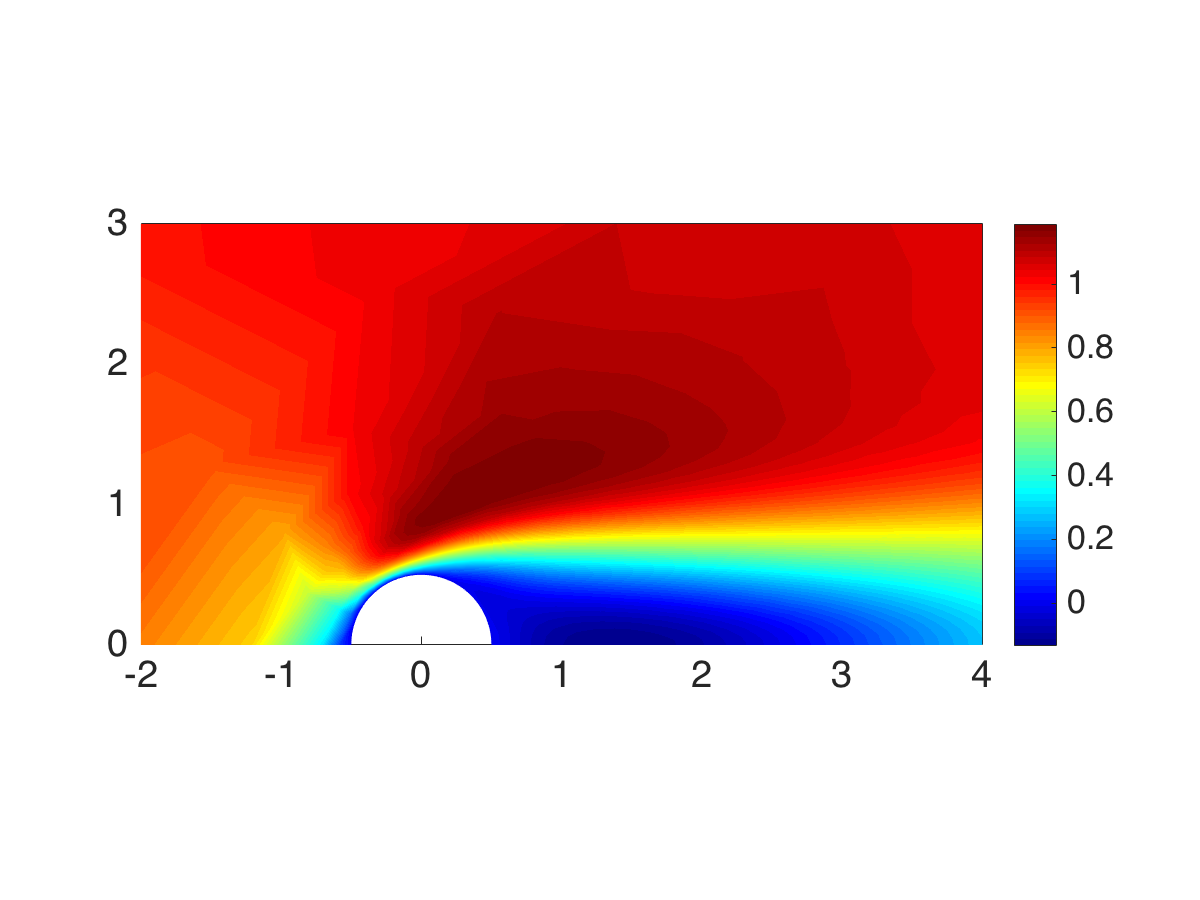
\includegraphics[width=.9 \linewidth]{Cylinder_MeanFlowRe60.png}
\end{center}
\caption{Structure of the {\em mean flow} over a cylinder for $Re = 
60$, as computed by the Self-Consistent model (streamwise velocity component).}
\label{fig:MF60}
\end{figure}



Figure \ref{fig:MF60} illustrates the structure of the mean flow for $Re=60$. As already identified by  \cite{MLugo2014}, the recirculation region associated with this mean flow is notably shorter than the one associated with the base flow (figure 2). 


%Line 19 shows how to plot the results along with the 

 
%\ref{HBEq0,HBEq1,HBphase}

Figure \ref{fig:HB_SC_DATA_COMP} shows the comparison between the WNL (green) and SC (red) models for the quantities of interest identified in this paper, namely the Strouhal number, the mean drag, the maximum lift, the energy-ampligude, and the recirculation length associated to the mean flow. When relevant, results concerning the base flow and the linear approach are also displayed (blue)
\footnote{Figure   \ref{fig:HB_SC_DATA_COMP} is obtained by line 19 of the script displayed in figure \ref{fig:listingNL}. The other figures are processed in a similar way. The entire set of commands to obtain all figures is provided in the script {\sf SCRIPT\_CYLINDER\_ALLFIGURES.m} .}.
Concerning the quantities $St$, $A_E$ and $L_x$, differences between SC, WNL models have already been commented in  \cite{MLugo2014} and \cite{FDR2016}. The predictions of the SC models were also compared to numerical simulations results showing excellent agreement in the range $Re \in [Re_c,100]$. Regarding the forces exerted on the body, we can remark that the predictions of the WNL and SC models rapidly depart from each other as soon as $Re-Re_c \gtrsim 1$. Comparison of these results with DNS simulations is not provided here (consistently with the objectives of the present paper) but the reader may verify that the SC model correctly predicts these quantities in the range of Reynolds number considered here.



%\clearpage

\section{Conclusion}
%The aim of the present review is to introduce advanced stability approaches 
%from a {\tt practical} point of view. The reader can reproduce all the figures presented 
%in this paper by just running the Matlab code available in the StabFem repository. 


The objective of this paper was twofold. First, we aimed at giving an up-to-date and comprehensive review on global stability approaches, both linear and nonlinear, including the most recent developments of the field. 
Secondly, we intended to provide an easy to use software performing all these computations from a single program. In accordance with this objective, all the figures presented in the paper can be produced by launching a single Matlab program available on the website of the project.

Although the focus here was on the reference case of 2D, incompressible flow around a cylinder, the  {\em StabFem } software is designed to be easily customisable to a variety of other situations. The project is currently in constant development, and incorporates a growing number of other configurations. In the present status, the project incorporates test-cases for the following classes of problems:
\begin{itemize}
\item Incompressible flows around 2D objects, either fixed or in movement such as the case of a spring-mounted cylinder \cite{Navrose},
\item Incompressible flows in axisymmetric geometries such as the wake of spheres and disks \cite{Tchoufag2015} and the flow through apertures \cite{FabreISMA}, 
\item Compressible flow around 2D objects  \cite{Fani2018}, 
\item Oscillations of hanging drops and liquid bridges \cite{Chireux2015}
\end{itemize}
The project is intended as collaborative, so anyone who wants to contribute is welcome !





%\section*{Acknowledgements}

%J. Tchoufag, J. Mougel, O. Marquet, D. Sipp, 


\appendix


%The problem can be set into weak form by multiplying by multiplying Eq. \ref{Newton2} by a test function ${\bf v}$ and the associated divergence constraint by a test function $q$. After a few integration by parts we are led to :

%SECTION TO BE COMPLETED.

%We have to explain the integration by parts of the viscous term.




%\begin{eqnarray}
%\label{NewtonWeak}
%&\forall ({\bf v};q), \\
%\displaystyle &\int \left[ {\bf v} \cdot {\cal C}( {\bf u}_b^g , \delta {\bf u}_b) +  \nabla  \cdot \delta {\bf u}_b q -\nabla  \cdot {\bf v} \delta p_b
%+ \frac{2}{Re} {\bf D}(\delta {\bf u}_b) : {\bf D}({\bf v}) \right]
%\nonumber
%\\
%\nonumber
%\displaystyle & + \int \left[ {\bf v} \cdot ( {\bf u}_b^g \cdot \nabla {\bf u}_b^g) 
%+ \nabla \cdot {\bf u}_b^g  q 
%- \nabla \cdot {\bf v} p_b^g
%+ \frac{2}{Re} {\bf D}({\bf u}_b^g) : {\bf D}({\bf v}) \right] = 0 
%\end{eqnarray}


\section{Mesh convergence : efficiency of mesh adaptation and effect of domain size}
\begin{figure}
%\vspace{-.5cm}\vspace{-.5cm}
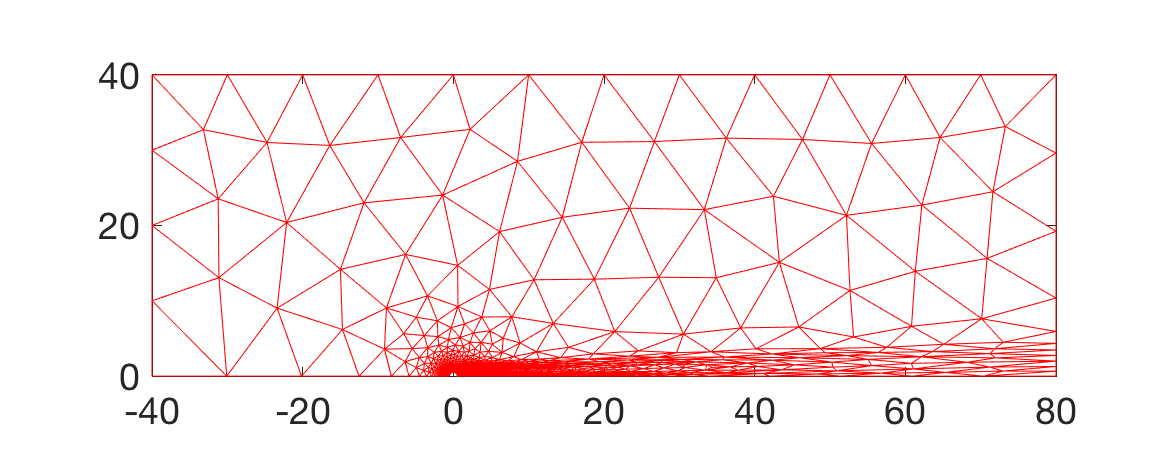
\includegraphics[width = .9\linewidth]{Cylinder_Mesh2_Full.png}
%\vspace{-.5cm}\vspace{-.5cm}
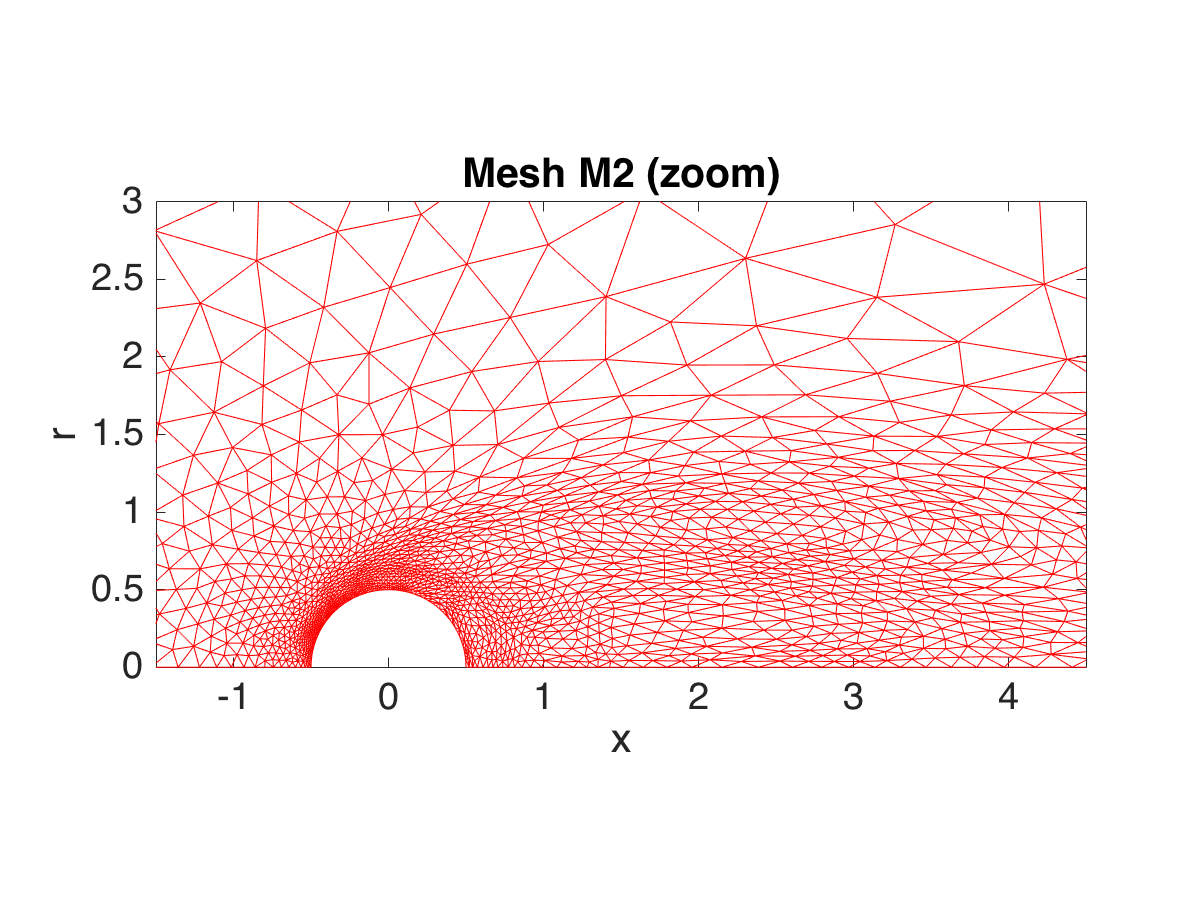
\includegraphics[width = .9\linewidth]{Cylinder_Mesh2.png}
\caption{Illustration of the stucture of mesh  $\mathbf{M}_2$ (adapted to both the base flow and structural sensitivity).}
\label{fig:mesh2}
\end{figure}

\begin{figure}
%\vspace{-.5cm}\vspace{-.5cm}
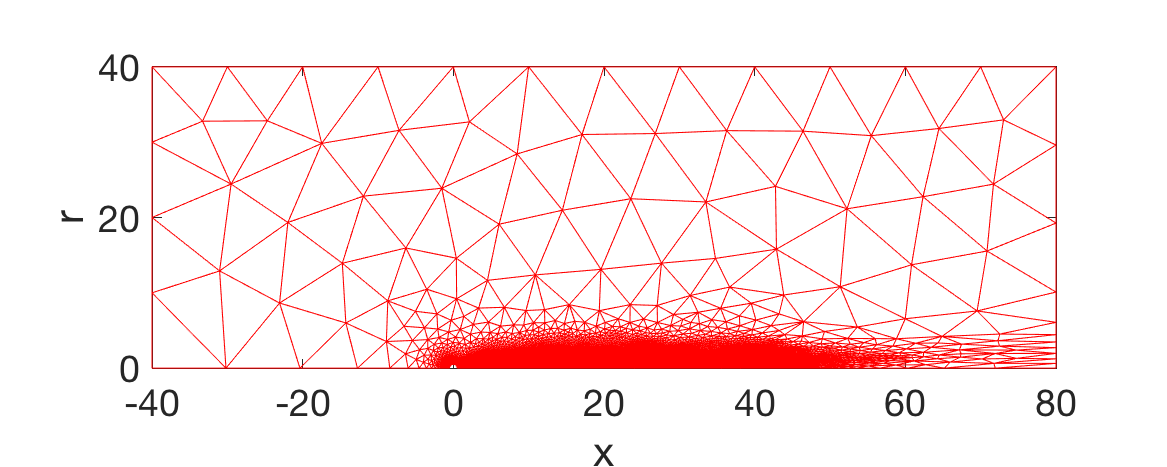
\includegraphics[width = .9\linewidth]{Cylinder_Mesh4_Full.png}
%\vspace{-.5cm}\vspace{-.5cm}
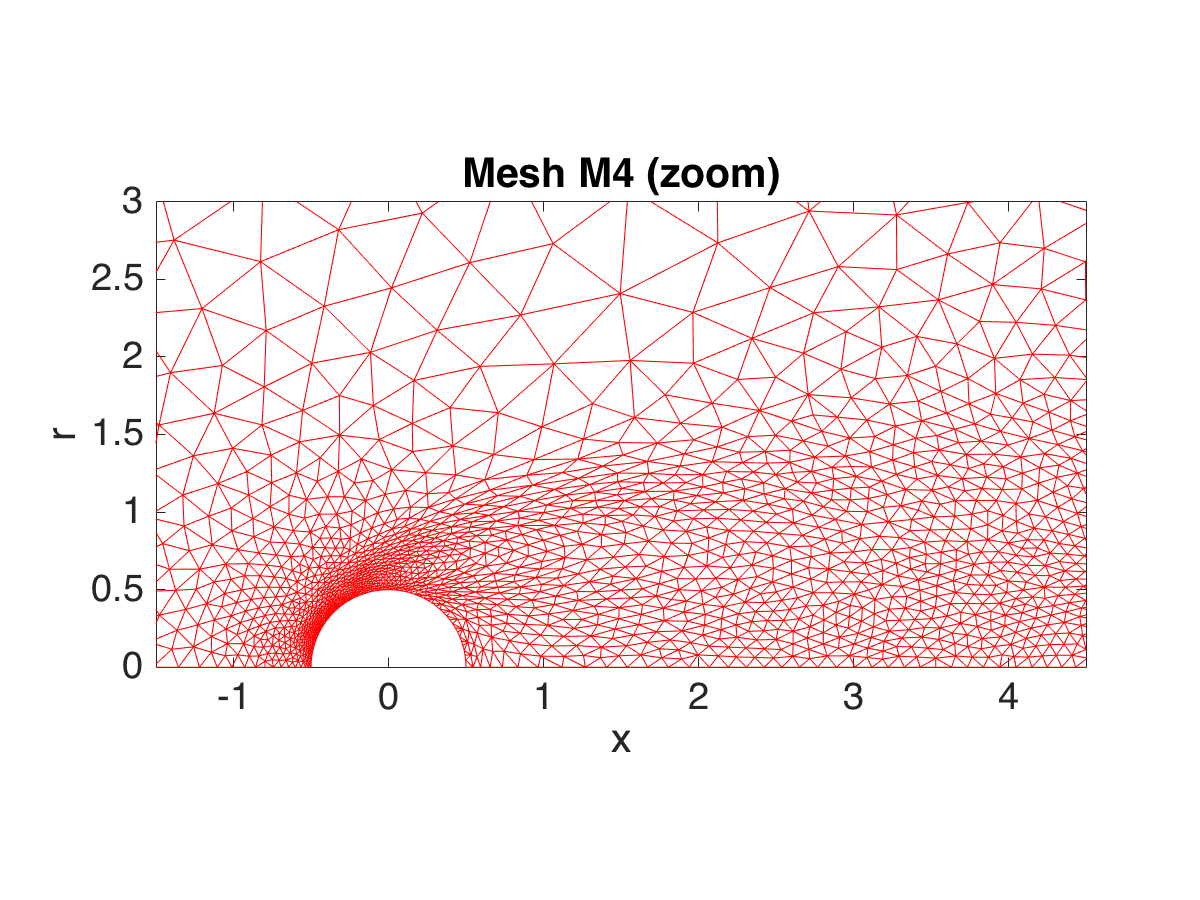
\includegraphics[width = .9\linewidth]{Cylinder_Mesh4.png}
\caption{Illustration of the stucture of mesh  $\mathbf{M}_4$ (adapted to both the base flow and direct eigenmode).}
\label{fig:mesh4}
\end{figure}



\begin{table*}
$$
\begin{array}{|c||c|c|c|c|c|c|c|c|c|}
\hline
\mbox{Mesh} & N_p & N_{dof} & \delta_{min} & \delta_{max} & \delta_A  & \delta_B  & \delta_C  & \delta_D  \\
\hline
\mathbf{M}_1 \mbox{(Adapt on base flow) } & 1429 & 12545	& 0.0131 & 14.33 		& 0.0259 	& 0.514 	& 0.819 	& 1.067 \\   
\mathbf{M}_2 \mbox{(Adapt on sensitivity) } & 2038 & 17885	& 0.0155 & 14.17 		& 0.02826 & 0.2046 	& 0.3909 	& 1.2014 	\\
\mathbf{M}_3 \mbox{(Adapt on sensitivity, split) } & 7974 & 70651	& 0.00786 & 7.131  		& 0.0104 	& 0.0744 	&   0.0975 & 0.614   \\
\mathbf{M}_4 \mbox{(Adapt on mode) } 	& 12080  & 103564		&0.00825	& 124.61		& 0.0229	& 0.143	& 0.0993	& 0.0934 \\
\mathbf{M}_5 \mbox{(Adapt on adjoint) } 	& 3813 	& 33715		& 0.0108	& 13.95		& 0.0176 	& 0.114	& 0.127	& 1.177  \\
\hline
\end{array}
$$
\caption{Description of meshes used for validation of mesh adaptation strategy : number of vertices $N_p$ ; number of degrees of freedom of the P2-P2-P1 Taylor-hood basis $N_{dof}$ ; cell size (minimum and maximum value, and value at four characteristic point A,B,C,D as defined in the text). 
 }
\label{tab:conv1}
\end{table*}


Fx = 0.6447; Lx = 4.0736
\begin{table*}
$$
\begin{array}{|c||c|c||c||c|c||c|c|c|}
\hline
\mbox{Mesh} & L_x & F_x & \lambda & L_{x,SC} & F_{x,SC} & \omega_{SC}  & F_{y,1,c} & A_{E} \\
\hline
\mathbf{M}_1 & 4.0733 & 0.64310	& 0.047056 + 0.74416i 		& 2.6073  & 0.69277 	&  0.84334 & 0.1298 & 1.8301  \\
\mathbf{M}_2 & 4.075 &.  0.64348  	& 0.046719 + 0.74489i 		& 2.6153  & 0.69246 	& 0.84351 & 0.12789 & 1.7134 \\  
\mathbf{M}_3 & 4.0772 & 0.64391 	& 0.04684. +  0.74511i 		& 2.6141  & 0.69338 	& 0.84383 & 0.12799 & 2.048   \\ 
\mathbf{M}_4 & 4.0748 & 0.64402 	& 0.04676  + 0.74502i 		& 2.6130 	& 0.69034 	& 0.84371 & 0.12809 & 2.5905 \\
\mathbf{M}_5 & 4.0736 & 0.64470	& 0.046782+0.74534i		& 2.6142 	& 0.69399		& 0.84390 & 0.12800 & 1.8234 \\
\hline
\end{array}
$$
\caption{Results for mesh adaptation strategy ($Re = 60$) : Base-flow characteristics $L_x$ and $F_x$, linear eigenvalue $\lambda$, 
Nonlinear self-consistent model characteristics  $\omega_{SC}$, $F_{y,1,c}$ and $A_E$. All the results can be optained using the matlab program
{\sf SCRIPT\_CYLINDER\_MESHCONVERGENCE.m}. }
\label{tab:conv2}
\end{table*}



This appendix presents complementary results obtained using various mesh designs. 
All the results can be obtained using the following program available on the StabFem website : 
{\sf SCRIPT\_CYLINDER\_MESHCONVERGENCE.m}.

\subsection{Efficiency of the mesh adaptation process}

As discussed in section 3, the mesh adaptation proves to be an extremely efficient way to obtain significant results 
with very reasonable meshes. The objective of this paragraph is to demonstrate this point by comparing the efficiency of several ways to perform mesh adaptation. 

For this purpose, 5 meshes were generated. 
Mesh $\mathbf{M}_1$ was adapted on the {\em base flow} obtained for $Re=60$.
Mesh $\mathbf{M}_2$ was adapted to both the base flow and structural sensitivity.
Mesh $\mathbf{M}_3$ was obtained by a subsequent refinement of mesh $\mathbf{M}_2$, splitting all triangles in four subtriangles, therefore doubling the effective density of the mesh.
Meshes $\mathbf{M}_4$ and $\mathbf{M}_5$ were obtained by adapting to the structure of the direct eigenmode and of the adjoint eigenmode.
In each case, the adaptmesh process was repeated twice in order to ensure a correct convergence.

Figures \ref{fig:mesh2} and \ref{fig:mesh4} illustrate the structure of meshes $\mathbf{M}_2$ and $\mathbf{M}_4$. As can be observed, these two mesh adaptation strategies lead to meshes with comparable densities in the region close to the cylinder. On the other hand, when moving downwards in the wake, mesh $\mathbf{M}_2$ quickly gets rather coarse, while mesh $\mathbf{M}_4$ maintains a significant density  

Table \ref{tab:conv1} gives numerical informations about the geometry of these meshes. In particular, we document the minimum and maximum cell size, as well as the cell size at four point A,B,C,D defined with by their coordinates as follows : $(x_A,y_A) = (0,0.5)$ (within the boundary layer at the cylinder wall); $(x_B,y_B) = (2.5,0.5)$ (in the region of maximum structural sensitivity); $(x_C,y_C) = (4,0)$ (in the near wake); $(x_D,y_D) = (10,0)$ (in the far wake). Results confirm that mesh all meshes have similar densities in the near wake (cell size at points A,B,C are comparable) 
while $\mathbf{M}_4$ has maximum resolution in the far wake (in the vicinity of point D).

Table  \ref{tab:conv2} compares the results obtained with the five meshes. For base-flow characteristics $L_x$ and $F_x$, all values agree with a relative dispersion of less than $0.15\%$, confiming that all adaptation stategies are successful to correctly compute the base flow. 
The performances of meshes for linear stability calculations can then be evaluated by comparing the eigenvalues. Meshes $\mathbf{M}_2$ to $\mathbf{M}_5$ all give values within less than $0.1\%$ dispersion. The value obtained with mesh  $\mathbf{M}_1$, which is not adapted to the eigenmode, is a bit farther from the others but still rather good. The table also displays results allowing to compare the performances of meshes for nonlinear self-consistent calculations. As for the frequency and the maximum lift, meshes $\mathbf{M}_2$ to $\mathbf{M}_5$ again give almost identical values within less than $0.1\%$ dispersion. The dispersion is much larger concerning the energy-amplitude of the perturbation $A_E$ displayed in the last column. Only the mesh $\mathbf{M}_4$ is able to correctly compute this quantities, while all other meshes significantly underestimate it. This is not surprising since this quantity is an integral one which depends upon the structure of the nonlinear perturbation in the whole wake, not only the near-wake region.

From this study we can conclude that if we are only interested in predicting the frequency of the mode and the forces exerted on the cylinder (in both linear and nonlinear regimes), the strategy of mesh adaptation to both base flow and structural sensitivity (mesh $\mathbf{M}_2$) is the most efficient and leads to a very light mesh (here only 2048 vertices). On the other hand, if we are interested in describing the structure of the perturbation in the whole domain (and being able to correctly evaluate its energy), mesh adaptation to the eigenmode structure is preferable. However this second strategy produces a much heavier mesh (here 12080 point).
 
 
 \begin{table*}
$$
\begin{array}{|c|c||c|c||c||c|c||c|c|}
\hline
\mbox{Mesh} & N & L_x & F_x & \lambda & L_{x,SC} & F_{x,SC} & \omega_{SC}  & F_{Y,SC} \\%& A_{E,SC} \\
\hline
%\mathbf{M}_2 \mbox{(ref)} 	& 7974  	& 4.0772 & 0.64391 	& 0.04684. +  0.74511i 	& 2.6141  & 0.69338 	& 0.84383 & 0.12799 & 2.048   \\ 
\mathbf{M}_6 [-20,40]x[0,20] 			& 1954	&  4.1097 & 0.65048 	& 0.048335+0.74989i 	& 2.6014  & 0.69988 & 0.85032 & 0.13219 \\%& 1.7019   \\ 
\mathbf{M}_7 [-80,160]x[0,80] 			& 2292	& 4.0618 & 0.64046		& 0.046081+0.74286i 	& 2.6188 	& 0.68924 	& 0.84042 & 0.12631 \\%& 1.6892 \\
\mathbf{M}_8 \mbox{("slip" conditions)}	 & 2026	& 4.0701 &0.64590		& 0.047017+0.74790i	& 2.6127 	& 0.69492		& 0.84613 & 0.12836 \\%& 1.7154 \\
\mathbf{M}_9 \mbox{("inlet" conditions)}	 & 2043	& 4.0677 &0.64	557	& 0.047077+0.74781i	& 2.6152 	& 0.69429		& 0.84562  & 0.12771 \\%1.7004 \\
\hline
\end{array}
$$
\caption{Comparison of the performances of several meshes with variable dimensions and different boundary conditions}
\label{tab:conv3}
\end{table*}






\subsection{Effect of domain size and boundary conditions}

As already identified in several previous studies, the size of the domain and the type of boundary conditions applied at the boundaries have a notable impact on the results. To illustrate this, we designed four additional meshes. All were obtained through adaptation to base flow and sensitivity, just as mesh $\mathbf{M}_2$.
Meshes $\mathbf{M}_6$ and $\mathbf{M}_7$ are respectively twice smaller and twice larger than the reference one. 
Meshes $\mathbf{M}_8$ and $\mathbf{M}_9$ have the same dimension but the boundary condition at the lateral boundary
 $\Gamma_{lat}$ differs. Unlike the reference case $\mathbf{M}_2$ which uses a no-stress boundary condition (identical to that applied at the outlet), mesh $\mathbf{M}_8$ uses a "slip" condition $u_y = 0 ; \partial u_x/\partial y = 0$ while mesh $\mathbf{M}_9$ uses an even more restrictive constant-flow condition (the condition at the lateral boundary is $u_x = 1, u_y = 0$, just as for the inlet).
 
Even though the domain size of the reference case (namely $[-40,80]\times[0,40]$) may appear large, the table shows that confinement effects are still present. The quantity which appears the most sensible to domain size and/or boundary conditions is the imaginary part of the linear eigenvalue. Interestingly, the nonlinear SC results appears to be more robust with respect to confinement effects than linear ones. 
In effect, values for nonlinear frequency $\omega_{SC}$ and the maximum lift $F_{y,1,c}$ obtained with meshes  $\mathbf{M}_2$, $\mathbf{M}_7$ $\mathbf{M}_8$ and $\mathbf{M}_9$ agree with less than $0.3\%$ dispersion.





\section{Additional details of the weakly nonlinear approach}

\subsection{Derivation of the amplitude equation using multiple-scale approach}

The initial derivation of \cite{SippLebedev} makes use of a multiple scale method in order to obtained an amplitude equation.
The starting point can be taken as the following expansion of the velocity flow field:
\be{WNL2}
\begin{aligned}
&{\bf u} = {}  {\bf u}_{bc} + \epsilon \left[ A_{wnl}(\tau)  \hat{\bf u} e^{i \omega_c t} + c.c. \right]\\
&+ \epsilon^2 \left[ {\bf u}_\epsilon + |A_{wnl}(\tau) |^2  {\bf u}_{2,0} + \left(  A_{wnl}(\tau) ^2 {\bf u}_{2,2} e^{2 i \omega_c t} + c.c. \right) \right]\\
& + {\cal O}( \epsilon ^3),
\end{aligned}
\ee
Note that compared to the simplified version given in the main text by eq. \ref{WNL1}, the amplitude $A_{wnl}$ depends upon a slow time scale 
$\tau = \epsilon^2 t$.

Substituting the expansion \ref{WNL2} into the Navier-Stokes equations \ref{NSprimitive} and grouping terms multiplied by the same power of $\epsilon$, a hierarchy of equations is obtained. The order $\epsilon^0$ gives directly the base flow at $Re_c$. The order $\epsilon^1$
corresponds to the linear neutral eigenmode as computed in the first part of this article.
The order $\epsilon^2$ contains three terms respectively computed as the solutions of the following linear problems:
\begin{eqnarray}
 {\cal LNS}_{{\bf u}_{bc}} ({\bf u}_\epsilon) - 2 \nabla \cdot {\mathsf D}({\bf u}_{bc}) &=&0,
\label{eq:LL1} \\
{\cal LNS}_{{\bf u}_{bc}} ({\bf u}_{2,0}) &=& {\cal C}(\hat{\bf u},\overline{\hat{\bf u}}), \label{eq:LL2} \\
{\cal LNS}_{{\bf u}_{bc}} ({\bf u}_{2,2}) - 2 i \omega_c {\bf u}_{2,2}  &=& \frac{1}{2} {\cal C}(\hat{\bf u},\hat{\bf u}). \label{eq:LL3}
 \end{eqnarray}

Finally, compatibility conditions, given by the Fredholm's alternative, are imposed at order $\epsilon^3$ to remove the secular terms, leading to an amplitude equation, known as Stuart-Landau equation:
\be{WNL3_2}
\frac{\partial A_{wnl}}{\partial \tau} = \Lambda A_{wnl} - (\nu_0+\nu_2)  |A_{wnl}|^2 A_{wnl},
\ee
where coefficients $\Lambda$, $\nu_0$ and $\nu_2$ are given by
\begin{eqnarray}
\Lambda &=& -\frac{ \left< {\hat{\bf u}}^\dag, 
\left( {\cal C}({\bf u}_\epsilon, \hat{\bf u}) + 2 \nabla \cdot  {\mathsf D}( \hat{\bf u}) \right) \right>}
{  \left<  \hat{\bf u}^\dag,\hat{\bf u} \right> },\label{LAMBDA}\\
\nu_0 &=& \frac{ \left< {\hat{\bf u}}^\dag,  {\cal C}({\bf u}_{20}, \hat{\bf u} ) \right>}
{  \left<  \hat{\bf u}^\dag,\hat{\bf u} \right> },\label{NU0}\\
\nu_2 &=& \frac{ \left< {\hat{\bf u}}^\dag,  {\cal C}({\bf u}_{22}, \overline{\hat{\bf u}})  \right>}
{  \left<  \hat{\bf u}^\dag,\hat{\bf u} \right> }.,\label{NU2}
 \end{eqnarray}


\subsection{Normalisation of the eigenmode}

\begin{table*}[!h]
\centering
$$
{\small
\begin{array}{|c||c|c|c|c|c|c|c|c|}
\hline
\mbox{Norm.} & \lambda & \nu_{0} & \nu_{2} &\omega_{\epsilon}& F_{x,0,\epsilon} & F_{y,1,c}/\epsilon & F_{y,1,s}/\epsilon &  |F_{y,1}| /\epsilon \\
\hline
\mbox{\cite{SippLebedev}} & 9.10988+3.28004i & 9.3996-32.0289i & -0.305116-0.866118i & 36.2307 
& 5.2848 & 0.0349973 & -0.536113 & 0.537254
\\
\mbox{\cite{FDR2016}} &  9.10988+3.28004i  & (0.488701 -1.66524 i) \times 10^{-3} & (-1.58635 - 4.50309i )\times 10^{-5} &36.2307
& 5.2848 & 0.537254 & 0 & 0.537254
\\
\mbox{\cite{Fabre2008}} & 9.10988+3.28004i & 32.62-111.152i & -1.05886-3.00574i & 36.2307
& 5.2848 & 0.537254 & 0 & 0.537254
\\
\hline
\end{array}
}
$$
\caption{Results of the WNL approach for three different choices of eigenmode normalization.}
\label{tab:WNL_coefs}
\end{table*}



A key issue in the weakly nonlinear expansion is that the definition of the amplitude depends upon a normalization choice of the eigenmodes. Several choices are possible. In the literature three possibilities have been used:
%\begin{itemize}
%\item 

First, \cite{SippLebedev} normalized the eigenmode by assuming a specified value to the $y$-component of the velocity at one point, namely:
\be{normsipp}
\hat{u}_y(1,0) = 0.4612.
\ee
The advantage of this choice is that the coefficients $\nu_0$ and $\nu_2$ have the same order of magnitude as the coefficient $\Lambda$.

%\item 
Secondly, \cite{FDR2016} proposed the following normalization choice:
\be{normFDR}
\int_\Omega |\hat{\bf u}|^2 d {\bf x}  = \frac{1}{2}.
\ee
This directly leads to $|A| = A_E$, so this normalisation seems equivalent to the previous one.
%{\color{red} The lift phase is not specified in \cite{FDR2016} and can be set to nil before the normalization.}

%\item 
Thirdly, following \cite{Fabre2008}, another convenient choice is to normalize the eigenmode with its lift 
force: 
\be{normfabre}
{{\cal D}_{Re_c}(\hat{\bf u},\hat{p}) }=\frac{1}{2}.
\ee
The advantage of this choice is that the amplitude $|A|$ is then an direct measure of the fundamental lift.
In effect, eq. \ref{lift_cos} directlty leads to $F_{y,1,c} = |A|$, $F_{y,1,s} = 0$. 


In our implementation of the WNL approach, we allowed to choose the normalization convention, as seen in line 3 of figure \ref{fig:listingNL}.
%%ATTENTION, si figure est actualisé, il faut actualiser la ligne
In table \ref{tab:WNL_coefs} we give the predictions of the WNL approach using the three normalization choices.
We can note that the coefficients $\nu_0$ and $\nu_2$ strongly depend on the normalization choice. On the other hand, the frequency deviation $\omega_\epsilon$ and the $\lambda$ coefficient, and the term $F_{x,0,\epsilon}$ related to the dependency of mean drag with deviation from the threshold are independent upon the normalization.

Considering the lift force, columns 7 and 8 of the table show that the different choices of normalization give different values for the coefficients $F_{1,y,c}$ and $F_{1,y,s}$. %This explains that the normalization choice fixes differently the phase of the cycle. 
However,  the sin-cos expansion of the lift force can be recast as 
$F_y =  (F_{y,1,c} \cos \omega t + F_{y,1,s} \sin \omega t ) =  |F_{y,1}|  \cos (\omega t + \varphi)$ 
with $ |F_{y,1}| =  \sqrt{F_{y,1,c}^2 + F_{y,1,s}^2}$. The last column of the table confirms that the three possible normalization choices effectively lead to the same values of $|F_{y,1}|$.


%\be{lift_explanation}

%= {\color{red}|A|} \left( {\color{red}\frac{1}{2}} e^{i \omega t} + c.c. \right)
%=   {\color{red}|A|} \cos (\omega t) ; \quad F_{y,1,{\color{red}s}} = 0. 
%\ee

%\end{itemize}





\section{Additional details about the self-consistent method}

The objective of this appendix is to provide additional details about the  SC model in its original form as given by \cite{MLugo2014}, and to explain the connection with the simpler version discussed in section 4.2. The full model is obtained by introducing the decomposition (\ref{SC}) into the Navier-Stokes equations, leading to :
\begin{subequations}\label{sc12}
\begin{eqnarray}
{\cal NS}(  {\bf u }_m ) - A^2 {\cal C}( \tilde{{\bf u }}_1, \overline{\tilde{\bf u }_1}) = 0, 
\label{sis1}
\\
(\sigma_{sc} + i \omega_{sc}) \tilde{{\bf u }}_1 =  {\cal LNS}_{{\bf u }_m}(\tilde{{\bf u }}_1 ).
\label{sis2}
\end{eqnarray}
\end{subequations}

Equation (\ref{sis1}) provides the mean flow field ${\bf u }_m$ while the 
pseudo-eigenpairs $(\lambda_{sc},  \tilde{{\bf u }}_1)$ can be computed by solving the eigenvalue problem (\ref{sis2}).
\cite{MLugo2014} Initially proposed a resolution method involving two imbricated loops, which is advantageaously replaced by
the direct Newton resolution of section 4.3. 

%The computed mode is normalized as $ || \tilde{{\bf u }}|| = 1/{\sqrt{2}}$
%is of the same form as  (\ref{HBEq1}) except that $i \omega$ is 
%replaced by $\sigma_{SC} + i \omega_{SC}$. 
% The mean flow is then governed by the same equation
%\ref{HBEq0}) written above, while $\tilde{{\bf u }}_1$ is the solution of an eigenvalue problem with the same form as  (\ref{HBEq1}) except that $i \omega$ is replaced by $\sigma_{SC} + i \omega_{SC}$.

The self-consistent model has the following properties:
\begin{itemize}
\item[-] For $ A \ll 1$ it is equivalent to the linear eigenvalue problem (\ref{LEP}), and the generalized eigenvalue coincides with the one predicted by linear stability : $\sigma_{SC} + i \omega_{SC} = \sigma_{lin} + i \omega_{lin}$.
\item[-] For $\sigma_{SC}=0$ (corresponding to a specific choice of the amplitude $A=A_{sc}$),  the expansion (\ref{SC}) is equivalent to 
the Fourier expansion \ref{eq:sc1} taken as the starting point in the present paper. 
\item[-] For $0<A<A_{sc}$, the resolution leads to a relation $\sigma_{SC}(A) ; \omega_{SC}(A)$
such that $0< \sigma_{SC}(A) < \sigma_{lin}$.
 Although in this case the expansion ({\ref{SC}}) cannot represent the flow for all $t$, Manti\v{c}-Lugo et al \cite{MLugo2014} argued that the relation between $\sigma_{SC}$ and $A$ can be used to build an amplitude equation which captures the transient approach to the limit cycle. 
\end{itemize}

Note that in our numerical implementation, the programs can actually be used to solve the SC model in the general case (with $\sigma\ne0$). 
This can be controlled by assigning a nonzero value to the optional parameter \verb|sigma| of the  {\sf SF\_SelfConsistent.m} Matlab function. The interested reader will find on the website of the {\em StabFem} project a program {\sf SCRIPT\_CYLINDER\_NONLINEAR.m} which computes $A$ as function of $\sigma$ for $Re=100$, yielding identical results as displayed in figure 3 of \cite{MLugo2014}.

\section{Details of the weak formulation}

In the presentation of the numerical methods in sections 2.1 and 2.2, and introduction of the {\em weak form}, we have omitted an important point, namely the issue of boundary conditions. In this appendix we explain more rigorously how the weak formulation is obtained. We consider here the full time-dependent nonlinear Navier-Stokes equations, but the treatment of the base-flow equations and the linearised equations is essentially the same.

Noting $\Gamma$ the boundary of the numerical domain, the latter can be decomposed in five parts : 
$\Gamma = \Gamma_{in} \cup \Gamma_{cyl} \cup \Gamma_{axis} \cup \Gamma_{out} \cup \Gamma_{lat}$. 
Noting $\sigma = 2 Re^{-1} {\bf D}({\bf u}) - p {\bf 1}$ the stress tensor, the relevant boundary conditions are as follows:
\begin{itemize}
\item On $\Gamma_{in}$ (inlet): ${\bf u} = {\bf e}_x$ (Dirichlet).
\item On $\Gamma_{cyl}$ (surface of the cylinder): ${\bf u} = {\bf 0}$ (Dirichlet).
\item On $\Gamma_{out}$ (outlet): $\sigma \cdot {\bf n} = {\bf 0}$ (Neumann). 
\item On $\Gamma_{lat}$ (lateral boundary):  $\sigma \cdot {\bf n} = {\bf 0}$ (Neumann). 
\item On $\Gamma_{axis}$ (symmetry plane): $u_y = 0$ and $\sigma_{xy} = 0$ (Mixed). 
\end{itemize}
We will introduce the following notation for integrals along any portion of the boundary $\Gamma_i$ of the product of two quantities $\phi_1, \phi_2$ (either scalar or vectorial) :
%$\left< \phi_1, \phi_2 \right>_{\Gamma_i} $:
$$
\left< \phi_1, \phi_2 \right>_{\Gamma_i} = \int_{\Gamma_i}  \overline{\phi}_1 \cdot \phi_2   \mbox{ d} \ell,
$$
Instead of the simplified version \ref{NSweak}, the more precise form of the weak formulation can be first written as follows:
\begin{eqnarray}
\label{NSweakFull}
\forall [{\bf v},q], &&\quad \partial_t \left< {\bf v}, {\bf u}\right> = \left< {\bf v} , {\cal NS} ({\bf u},p) \right> + \left< q, \nabla \cdot {\bf u}\right>\\
+ &&\frac{1}{\epsilon} \left(  \left< {\bf v}, \bf{u} \right>_{\Gamma_{cyl}} + \left< {\bf v}, ({\bf u}- {\bf e}_x ) \right>_{\Gamma_{in}} 
+ \left< v_y, u_y\right>_{\Gamma_{axis}} \right) \nonumber \\
+ && \left< {\bf v}, \sigma \cdot {\bf n} \right>_{\Gamma_{out} \cup  \Gamma_{lat} \cup \Gamma_{axis} }  \nonumber 
\end{eqnarray}
where $\epsilon=10^{-30}$ is a small parameter used to impose the Dirichlet boundary conditions by penalization.
An integration by parts of the pressure gradient and viscous stress terms of the Navier-Stokes equation eventually 
leads to the weak form effectively used in the programs {\sf Newton2D.edp} and {\sf Stab2D.edp}:
\begin{eqnarray}
\forall [{\bf v},q], &&\, \partial_t \left< {\bf v}, {\bf u}\right> = - \left< {\bf v} , {\cal C}({\bf u},{\bf u})/2 \right>
- 2 Re^{-1} \left< {\mathsf D}({\bf v}) : {\mathsf D}({\bf u})  \right>  \nonumber \\
+ &&\left< \nabla \cdot {\bf v}, p \right> + \left< q, \nabla \cdot {\bf u} \right> \label{NSweakFullN} \\
+ &&\frac{1}{\epsilon} \left(  \left< {\bf v}, \bf{u} \right>_{\Gamma_{cyl}} + \left< {\bf v}, ({\bf u}- {\bf e}_x ) \right>_{\Gamma_{in}} 
+ \left< v_y, u_y\right>_{\Gamma_{axis}} \right) \nonumber 
\end{eqnarray}
Note that the Neumann boundary conditions do not appear any more thanks to the integration by parts.






%In this appendix we compare the results obtained with 8 different meshes, to demonstrate the efficency of the mesh adaptation process. The whole results can be obtained using the script {\em SCRIPT\_CYLINDER\_MESHCONVERGENCE.m} available in the StabFem repository.

%Giannetti \& Luchini\cite{GiannettiLuchini} showed that the accuracy of the stability results for the flow past a circular cylinder is strictly related to the mesh characteristics  in the wavemaker region, i.e. the region where the structural sensitivity reaches its maximum values. Following this idea, we chose as reference solution the field, computed on an adapted mesh obtained by using the structural sensitivity field.We set the interpolation  error equal to 0.01 and the size of the computational domain is $[-40,120]\times[0,40]$. The base flow is computed by using classical no-slip boundary conditions on the body surface, a uniform velocity profile at the inlet and no-stress boundary conditions at the outlet and lateral boundaries. The conditions for the stability computations are simply derived from the ones of the base flow.

%Figure \ref{fig:MeshConvergence} displays global stability results. We note that there is a very weak variation in the growth rate and we found an error up to 1\% on the  Strouhal number. Figure \ref{ill_bsflow} illustrate the procedure adopted to compute the 
%base flow and the adapted mesh. Figure \ref{stabmesh} reports the Matlab code 
%adopted to adapt the mesh by using the information provided by both the base flow and the sensitivity field. 



%Figure 1 gives a retranscription of the sequence of commands (from {\em SCRIPT\_CYLINDER\_ADAPTMESH\_BASEFLOW}) 
%and the output produced.

\bibliographystyle{asmems4}

\bibliography{ARTICLE_ASME}

\end{document}
